\chapter{Kretsar}

\section[Serie och parallellt]{Komponenter i serie och parallellt}

\subsection{Seriekopplade resistorer}
\textbf{HAREC
  a.\ref{HAREC.a.3.1.1a}\label{myHAREC.a.3.1.1a},
  a.\ref{HAREC.a.3.1.2}\label{myHAREC.a.3.1.2a},
  a.\ref{HAREC.a.3.1.3}\label{myHAREC.a.3.1.3a},
}
\index{resistor!seriekopplade}
\index{seriekoppling!resistorer}

\begin{wrapfigure}{R}{0.5\textwidth}
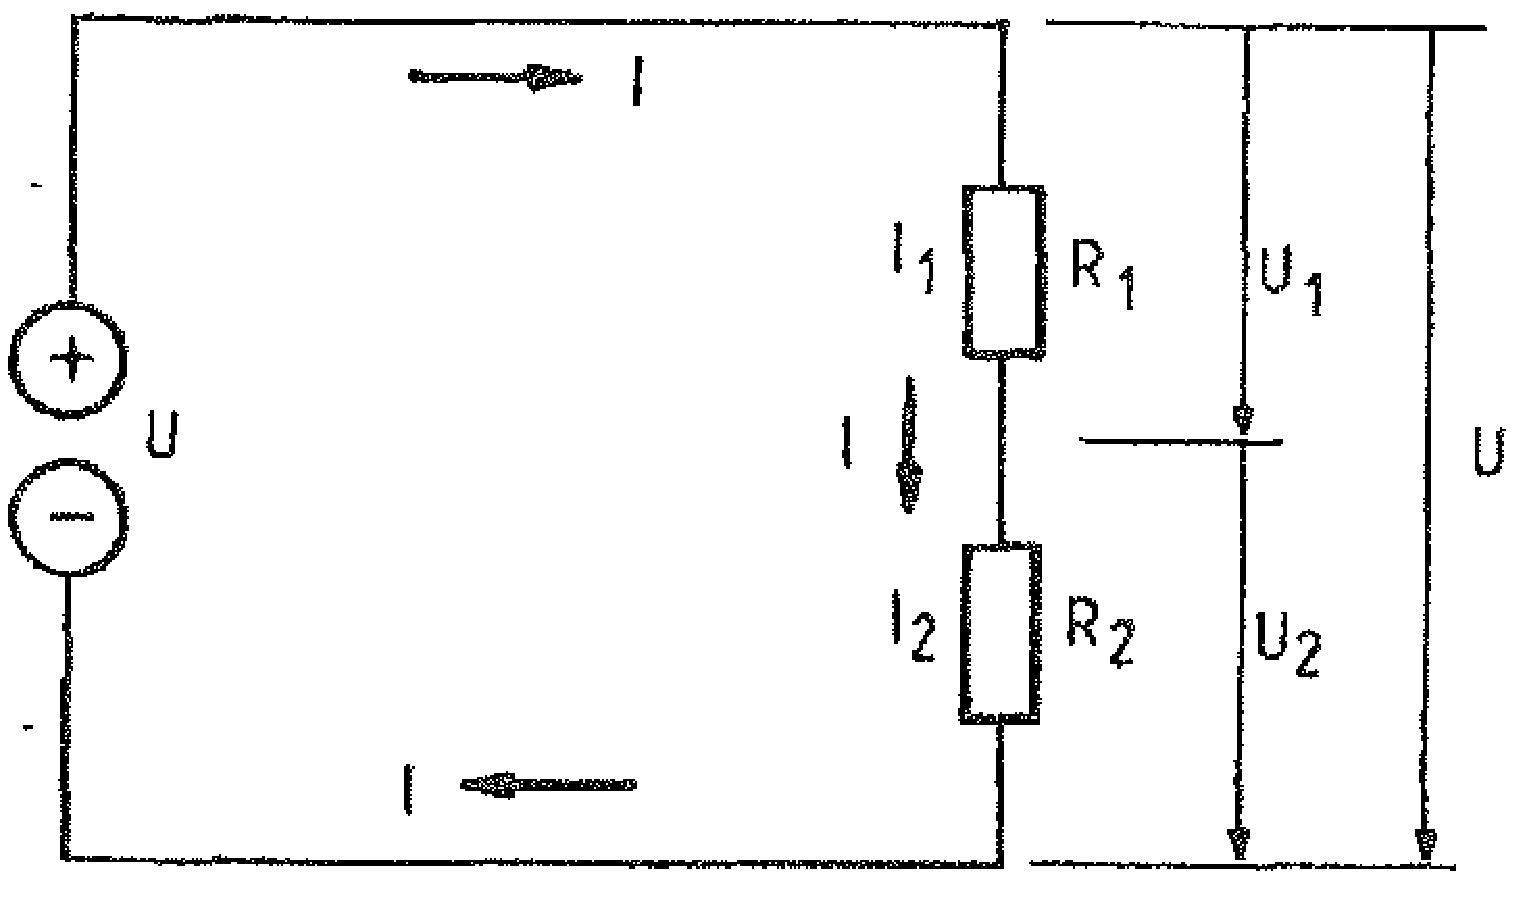
\includegraphics[width=0.5\textwidth]{images/cropped_pdfs/bild_2_3-01.pdf}
\caption{Seriekopplade resistorer}
\label{fig:BildII3-01}
\end{wrapfigure}

Bild \ref{fig:BildII3-01} visar seriekopplade resistorer.
Den totala resistansen av seriekopplade resistorer är summan av resistanserna.

\[R = R_1 + R_2 + R_3 \cdots \]

Strömmen är lika stor genom alla seriekopplade resistorer i strömvägen (ingen
avgrening).

\[I = I_1 = I_2 = I_3 \cdots \]

Den totala spänningen över seriekopplade resistorer är summan av spänningen över
var och en av dem.

\[U = U_1 + U_2 + U_3 \cdots \]

Spänningen över var och en av seriekopplade resistorer förhåller sig som deras
resistanser. För två resistorer gäller

\[\dfrac{U_1}{U_2} = \dfrac{R_1}{R_2}\]


\subsection{Parallellkopplade resistorer}
\textbf{HAREC a.\ref{HAREC.a.3.1.1b}\label{myHAREC.a.3.1.1b}}
\index{resistor!parallellkopplade}
\index{parallellkoppling!resistorer}

\begin{wrapfigure}{R}{0.5\textwidth}
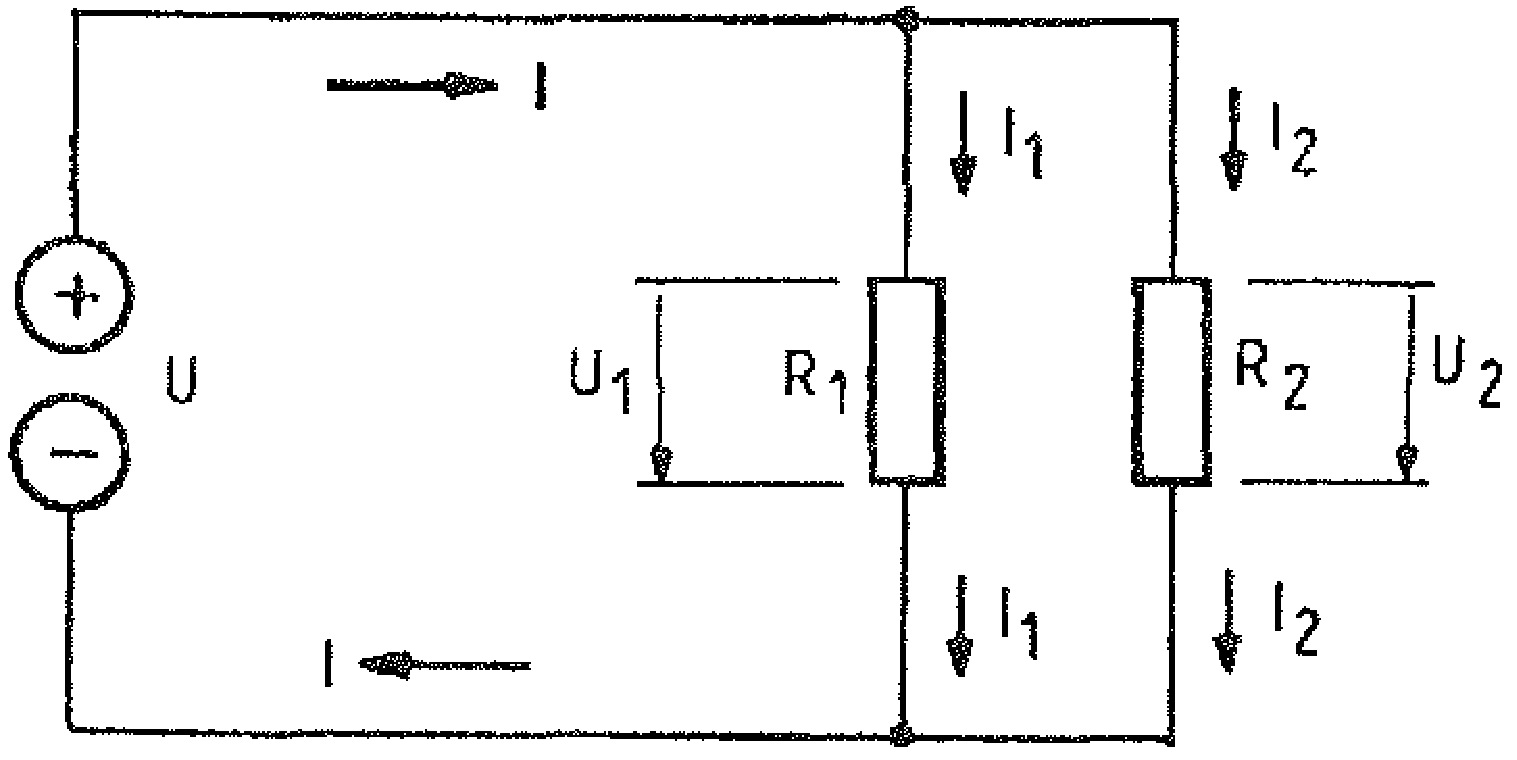
\includegraphics[width=0.5\textwidth]{images/cropped_pdfs/bild_2_3-02.pdf}
\caption{Parallellkopplade resistorer}
\label{fig:BildII3-02}
\end{wrapfigure}

Bild \ref{fig:BildII3-02} visar parallellkopplade resistorer.
Den totala resistansen av parallellkopplade resistorer är lägre än den lägsta
enstaka resistansen.

\[
\frac{1}{R} = \frac{1}{R_1} + \frac{1}{R_1} +
\frac{1}{R_2} + \frac{1}{R_3} + \cdots \frac{1}{R_n}
\]

För två resistorer gäller

\begin{align*}
\frac{1}{R} &= \frac{1}{R_1} + \frac{1}{R_2} && eller \\
R &= \frac{R_1 \cdot R_2}{R_1 + R_2}
\end{align*}

För tre resistorer gäller

\begin{align*}
\frac{1}{R} &= \frac{1}{R_1} + \frac{1}{R_2} + \frac{1}{R_3} && eller \\
R &= \frac{R_1\cdot R_2\cdot R_3}{R_1\cdot R_2 + R_1\cdot R_3 + R_2\cdot R_3}
\end{align*}

Strömmen förgrenar sig mellan parallellkopplade resistorer.
Den totala strömmen är summan av grenströmmarna

\( I = I_1 + I_2 + \cdots I_n \)

Spänningen är lika stor över resistorerna

\(U = U_1 = U_2 = U_3 = \cdots U_n \)

Grenströmmarna genom parallellkopplade resistorer fördelar sig omvänt
proportionellt mot deras respektive resistanser.
För två resistorer gäller

\[\frac{I_1}{I_2} = \frac{R_2}{R_1}\]

\subsection{Spänningsdelare}
\index{spänningsdelning}

\begin{wrapfigure}[18]{R}{0.5\textwidth}
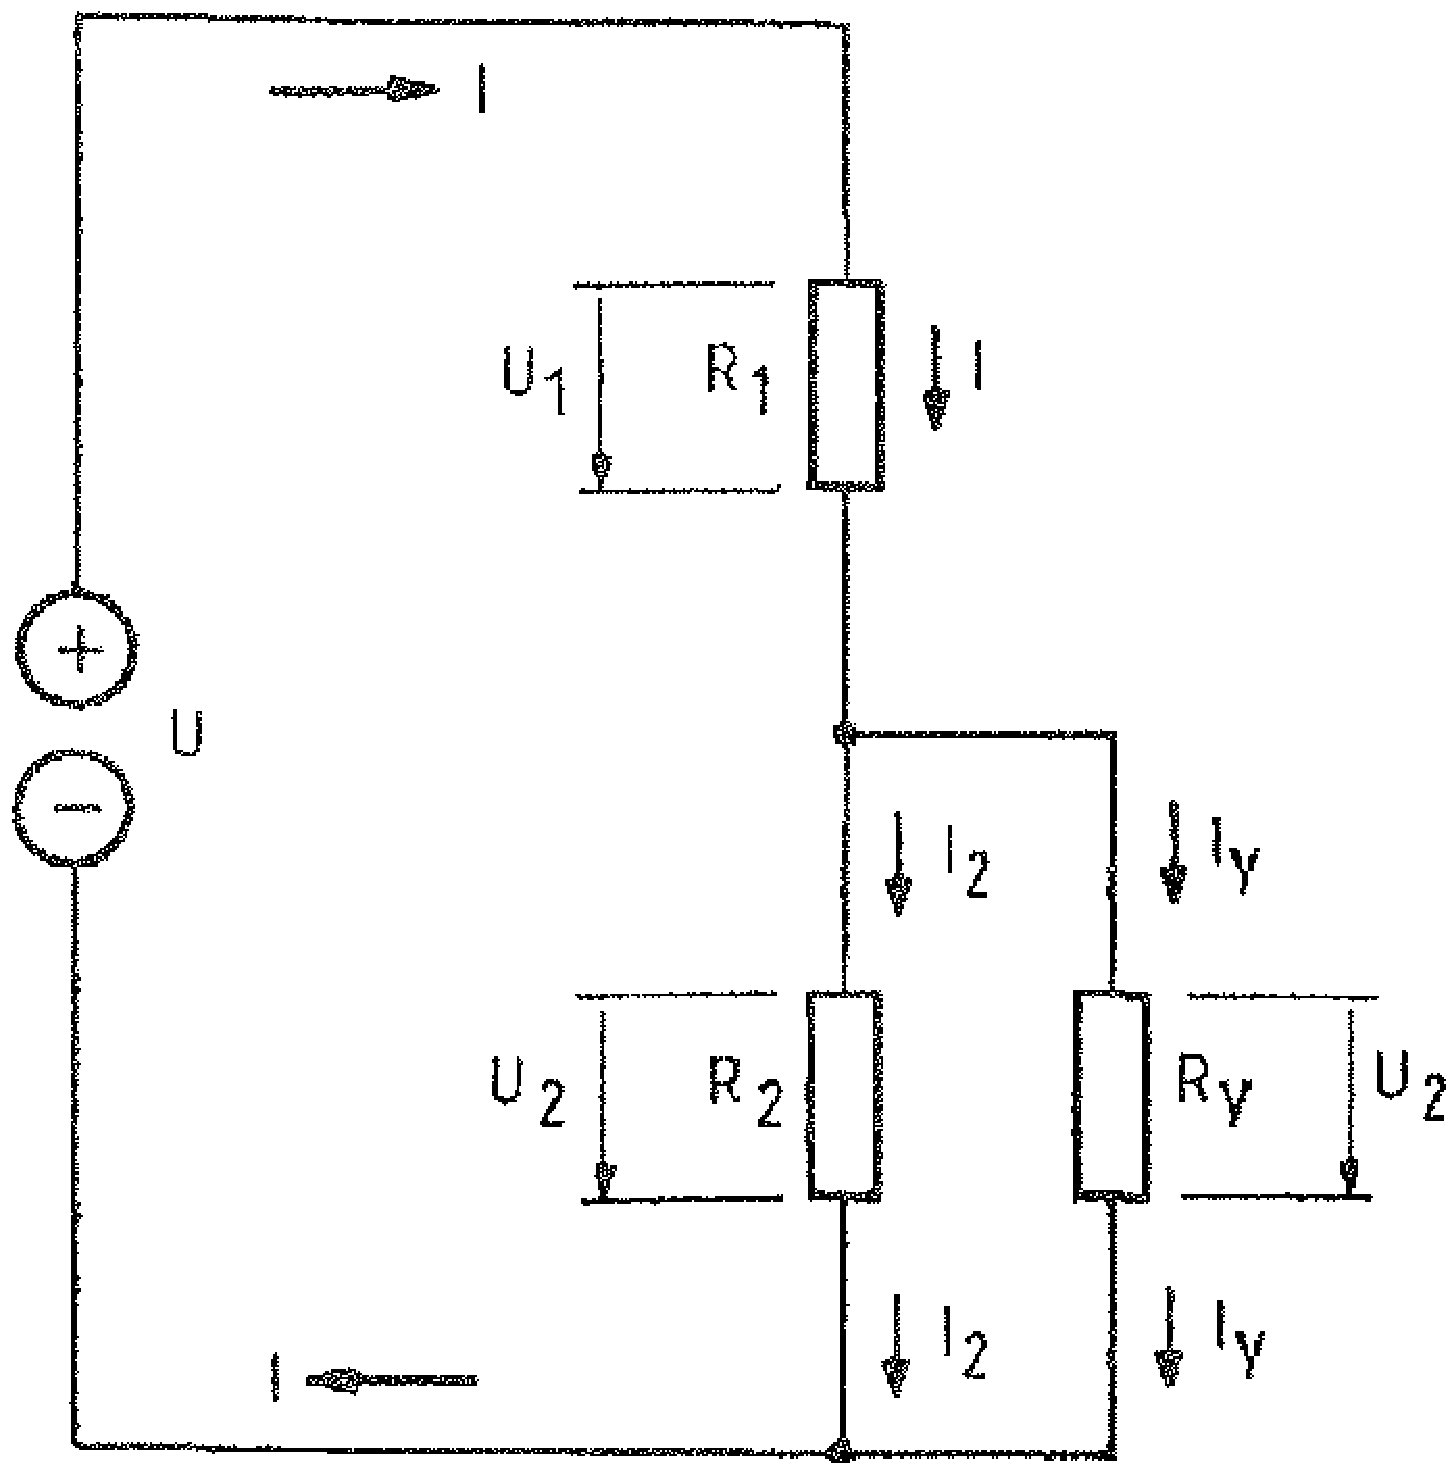
\includegraphics[width=0.5\textwidth]{images/cropped_pdfs/bild_2_3-03.pdf}
\caption{Resistiv spänningsdelare}
\label{fig:BildII3-03}
\end{wrapfigure}

Spänningsdelare förekommer i flera former.
Bild \ref{fig:BildII3-03} visar en spänningsdelare med resistorer där
spänningen \(U\) delas upp i spänningen \(U_1\) över resistorn \(R_1\)
respektive \(U_2\) över \(R_2\).
Man kan då till exempel använda spänningen för något ändamål.

Ett alternativ till spänningsdelning med resistorer med fasta värden är
\emph{potentiometern}. Det är en variabel spänningsdelare i form av en resistor
med ett uttag som kan flyttas mellan ändanslutningarna.

Om man nu ansluter en apparat parallellt över \(R_2\), till exempel ett instrument
vars inre resistans motsvaras av \(R_y\), så kommer spänningarna över \(R_1\)
och \(R_2\) att påverkas.

Om \(R_y\) är mycket större än \(R_2\), så kan man bortse från påverkan.
För att beräkna \(U_2\) kan man då använda följande formel för en obelastad
resistiv spänningsdelare.

\begin{align*}
\frac{U_2}{R_2} &= \frac{U}{R_1 + R_2} \quad \text{eller} \\
U_2 &= U \cdot \frac{R_2}{R_1 + R_2}
\end{align*}

Om \(R_y\) däremot är av samma storleksordning eller lägre än \(R_2\), så måste
man för att beräkna \(U_2\) använda en formel för en belastad resistiv
spänningsdelare, till exempel

\[
U_2 = U \cdot \dfrac{ \dfrac{R_2 \cdot R_y}{R_2 + R_y} }{ R_1 + \dfrac{R_2 \cdot R_y}{R_2 + R_y} }
\]

Härav förstås att till exempel en spänningsmätning ger olika resultat beroende
på den inre resistansen i voltmetern.

\subsection{Wheatstones brygga}
\index{Wheatstones brygga}

\begin{wrapfigure}[18]{R}{0.5\textwidth}
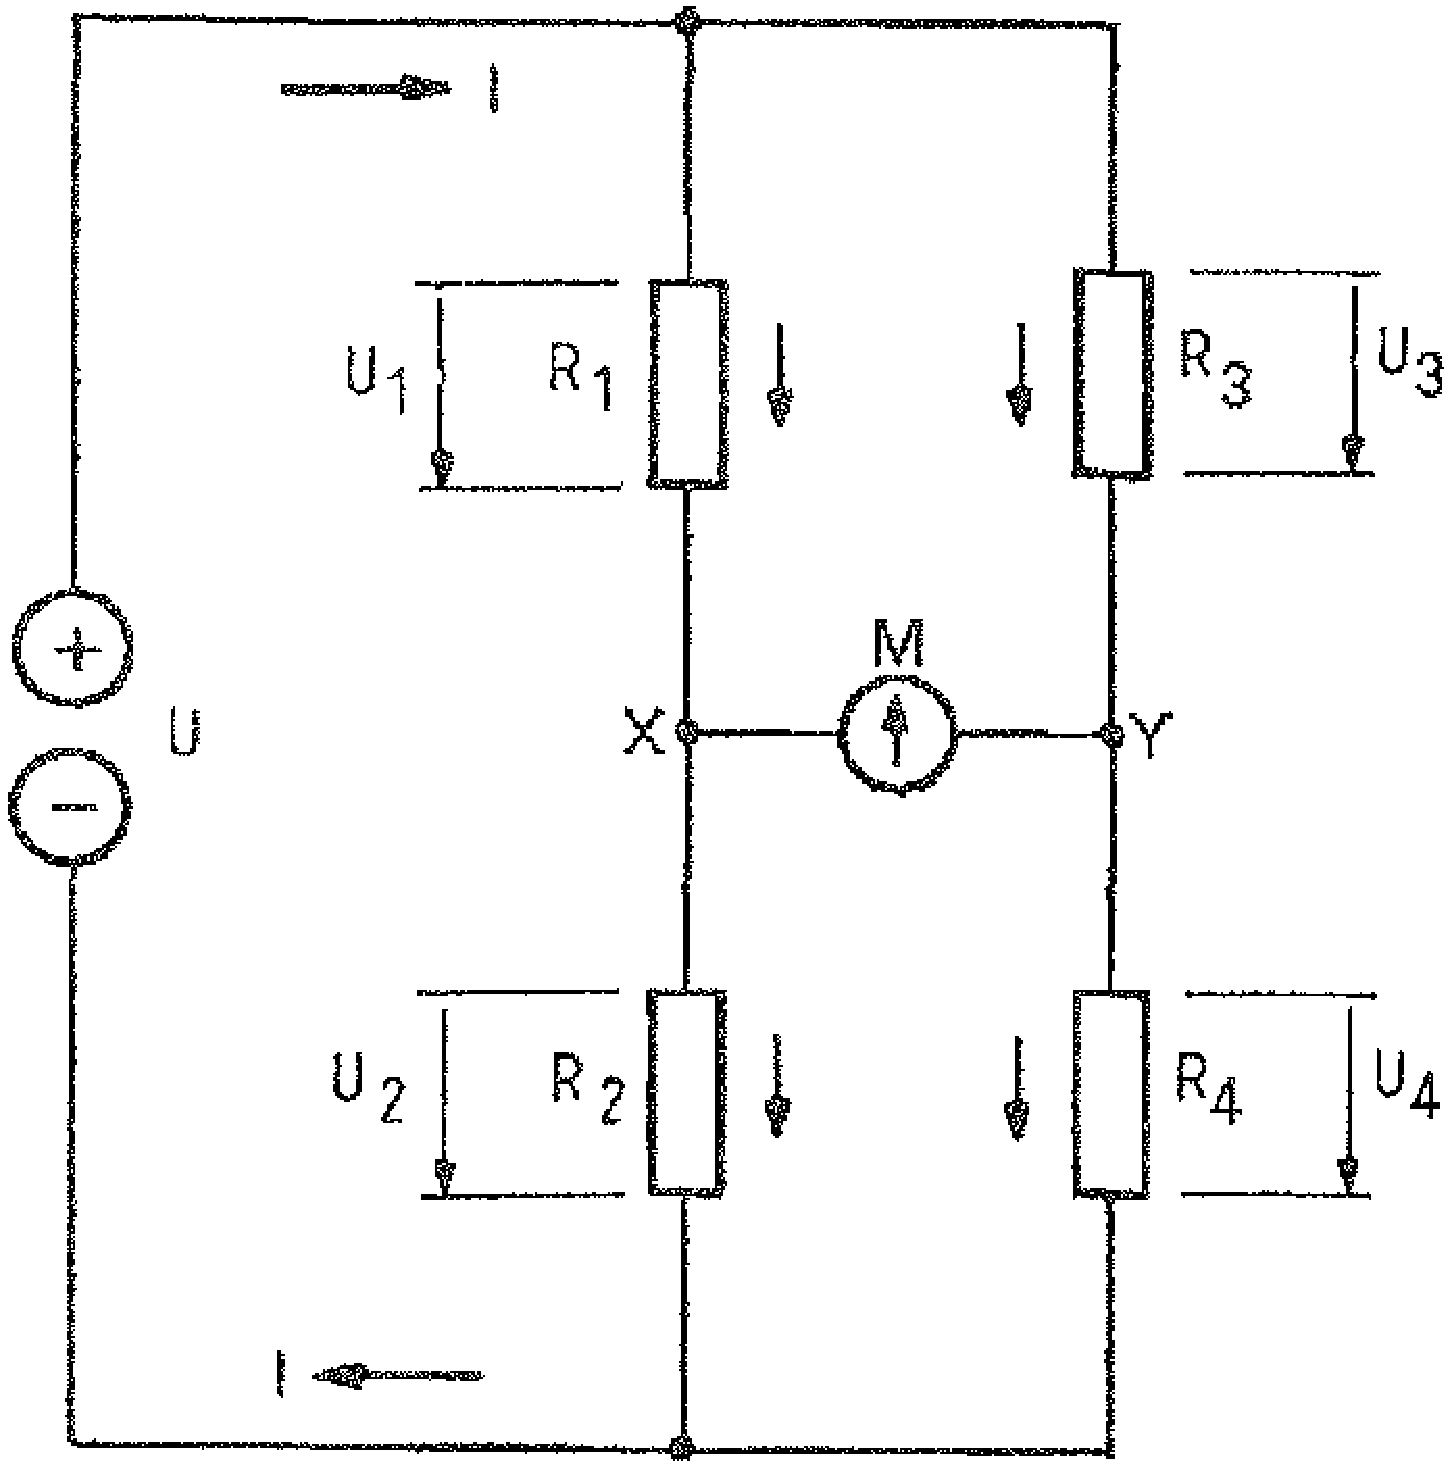
\includegraphics[width=0.5\textwidth]{images/cropped_pdfs/bild_2_3-04.pdf}
\caption{Wheatstones brygga}
\label{fig:BildII3-04}
\end{wrapfigure}

Bild \ref{fig:BildII3-04}

En speciell tillämpning av spänningsdelare är en \emph{Wheatstones brygga},
som används för att jämföra spänningar.

Bryggan kan ses som två parallellkopplade spänningsdelare varav den ena är en
potentiometer med en skala graderad till exempel i \(\Omega\).
Den andra spänningsdelaren består av en resistor med känd resistans och en
resistor med okänd resistans, det vill säga mätobjektet.

I ledningen som förbinder de respektive mittuttagen X och Y, finns en
amperemeter som nollströmsindikator.

Det flyter ström mellan X och Y när det finns en potentialskillnad -- spänning
-- däremellan.
Bryggan är då i obalans.
Det flyter däremot ingen ström där när det inte finns en potentialskillnad,
det vill säga när bryggan är i balans.
Balans (mätvärdet) får man genom justering av den graderade potentiometern
till noll ström.
Då gäller sambandet

\[\frac{R_1}{R_2} = \frac{R_3}{R_4}\]

Spänningsdelare och bryggor har tagits med för att påvisa att apparater
påverkar varandra när de kopplas samman, vilket är fallet även vid mätningar.

Spänningsdelning kan även utföras med kondensatorer och induktorer förutsatt
att det är fråga om en växelströmskrets.

\subsection{Parallellkopplade kondensatorer}
\textbf{HAREC a.\ref{HAREC.a.3.1.1f}\label{myHAREC.a.3.1.1f}}
\index{kondensator!parallellkopplade}
\index{parallellkoppling!kondensatorer}

\begin{figure*}[ht]
\begin{center}
  %%\begin{wrapfigure}[18]{R}{0.5\textwidth}
  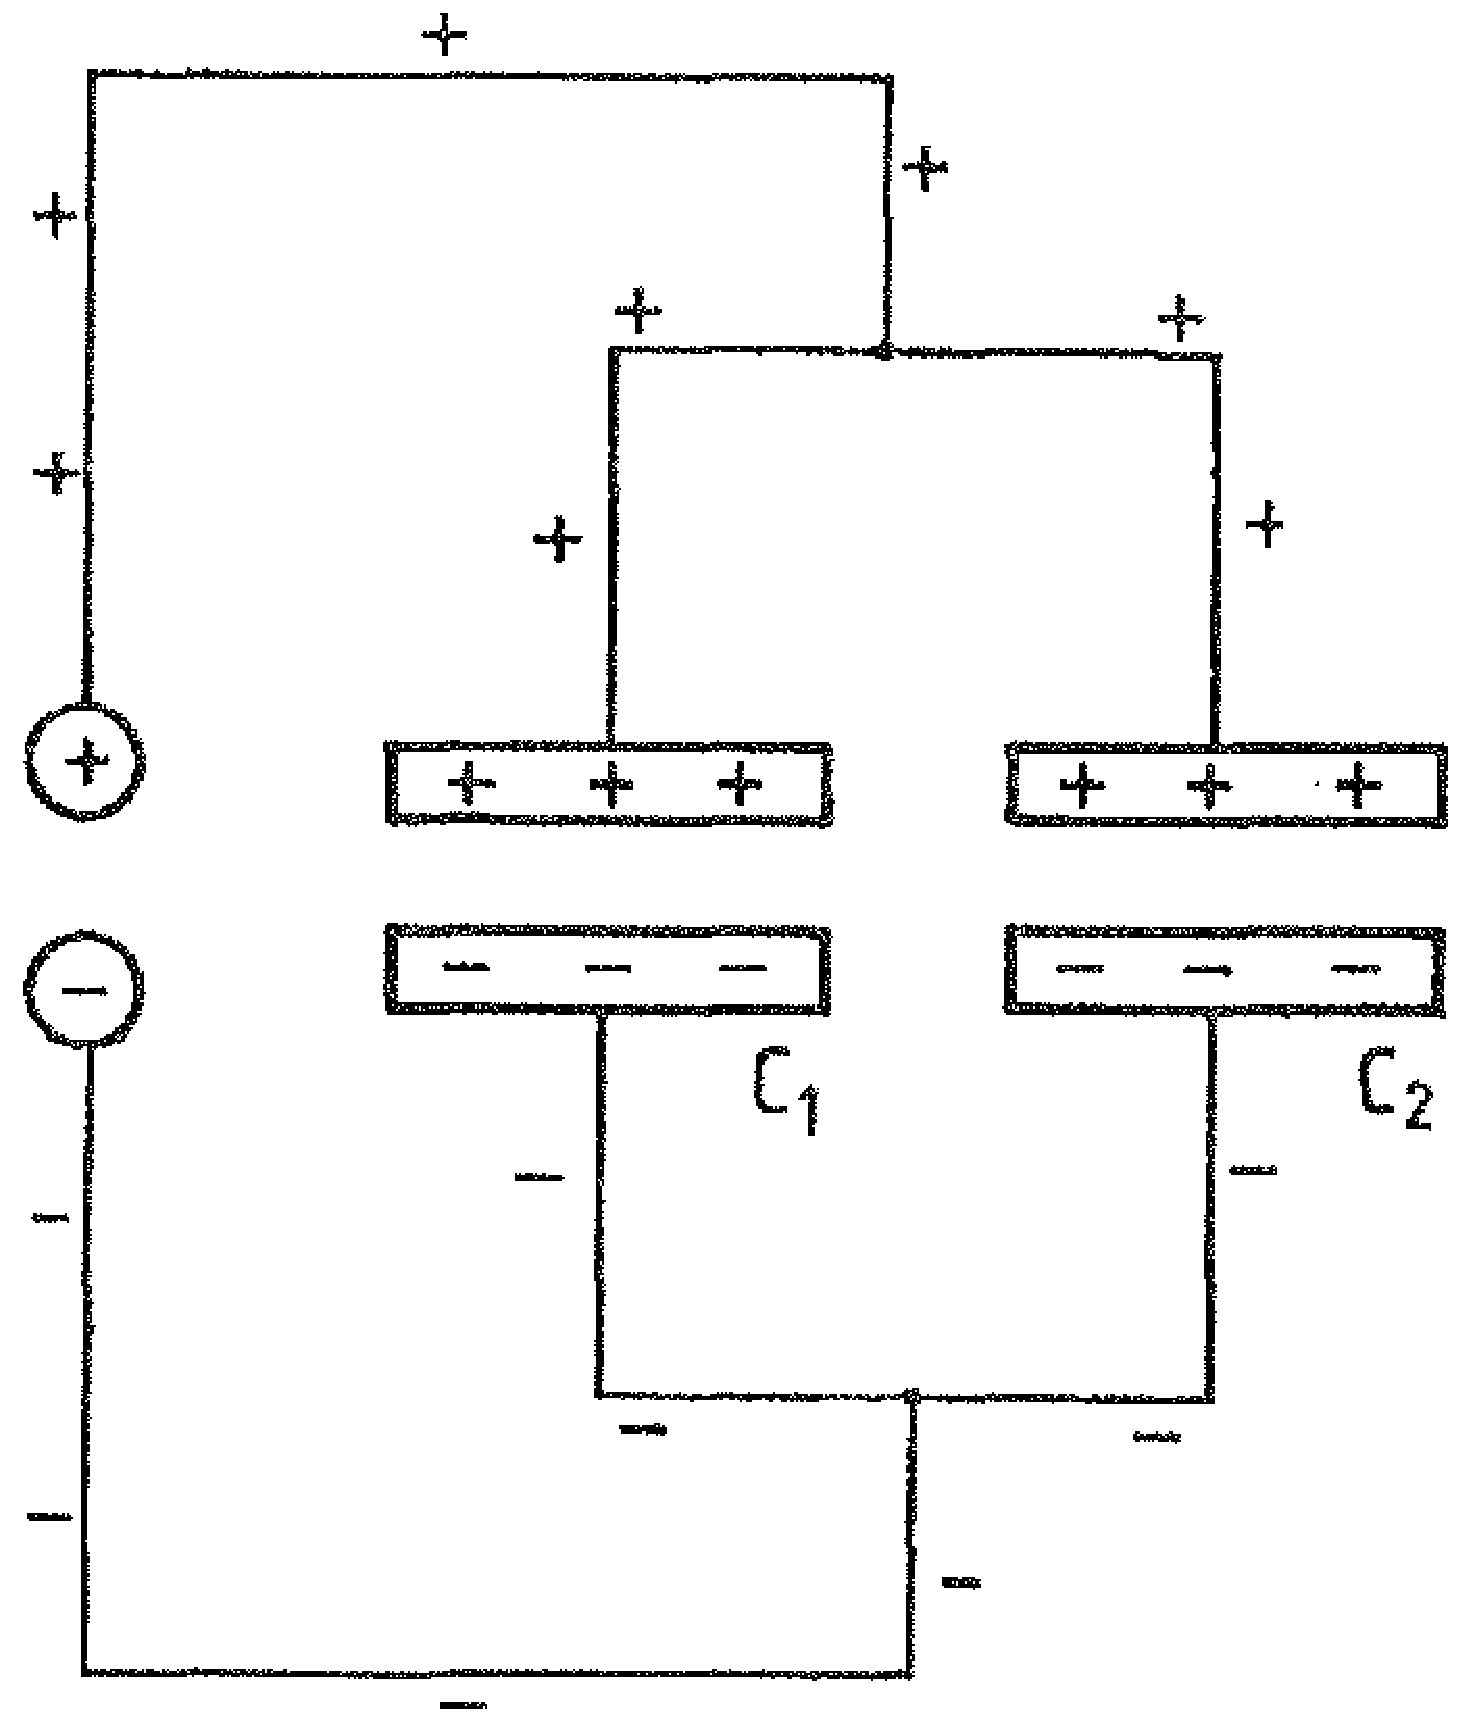
\includegraphics[width=0.5\textwidth]{images/cropped_pdfs/bild_2_3-05.pdf}
  \caption{Parallellkopplade kondensatorer}
  \label{fig:BildII3-05}
  %%\end{wrapfigure}
\end{center}
\end{figure*}

Bild \ref{fig:BildII3-05} visar parallelkopplade kondensatorer.
I stället för att använda en enda kondensator kan man parallellkoppla flera
kondensatorer för att uppnå önskad total kapacitans.

Den totala kapacitansen för parallellkopplade kondensatorer är summan av de
enskilda kapacitanserna.

\[C = C_1 + C_2 + C_3 + \cdots C_n\]

\textbf{Räkneexempel:}
\begin{enumerate}
\item \(C_1 = 5\ \mu F \quad C_2 = 10\ \mu F \quad C =\ ?\)
  \begin{align*}
    C &= C_1 + C_2 \\
    &= 5 + 10 \\
    &= 15\ \mu F
  \end{align*}
\item \(C_1 = 1\ nF \quad C_2 = 5\ pF \quad C =\ ?\)
  \begin{align*}
    C &= C_1 + C_2 \\
    &= 1 + 0,005 \\
    &= 1,005\ nF
  \end{align*}
\end{enumerate}

\subsection{Seriekopplade kondensatorer}
\textbf{HAREC a.\ref{HAREC.a.3.1.1e}\label{myHAREC.a.3.1.1e}}
\index{kondensator!seriekopplade}
\index{seriekoppling!kondensatorer}

\begin{figure*}[ht]
\begin{center}
  %%\begin{wrapfigure}[10]{R}{0.5\textwidth}
  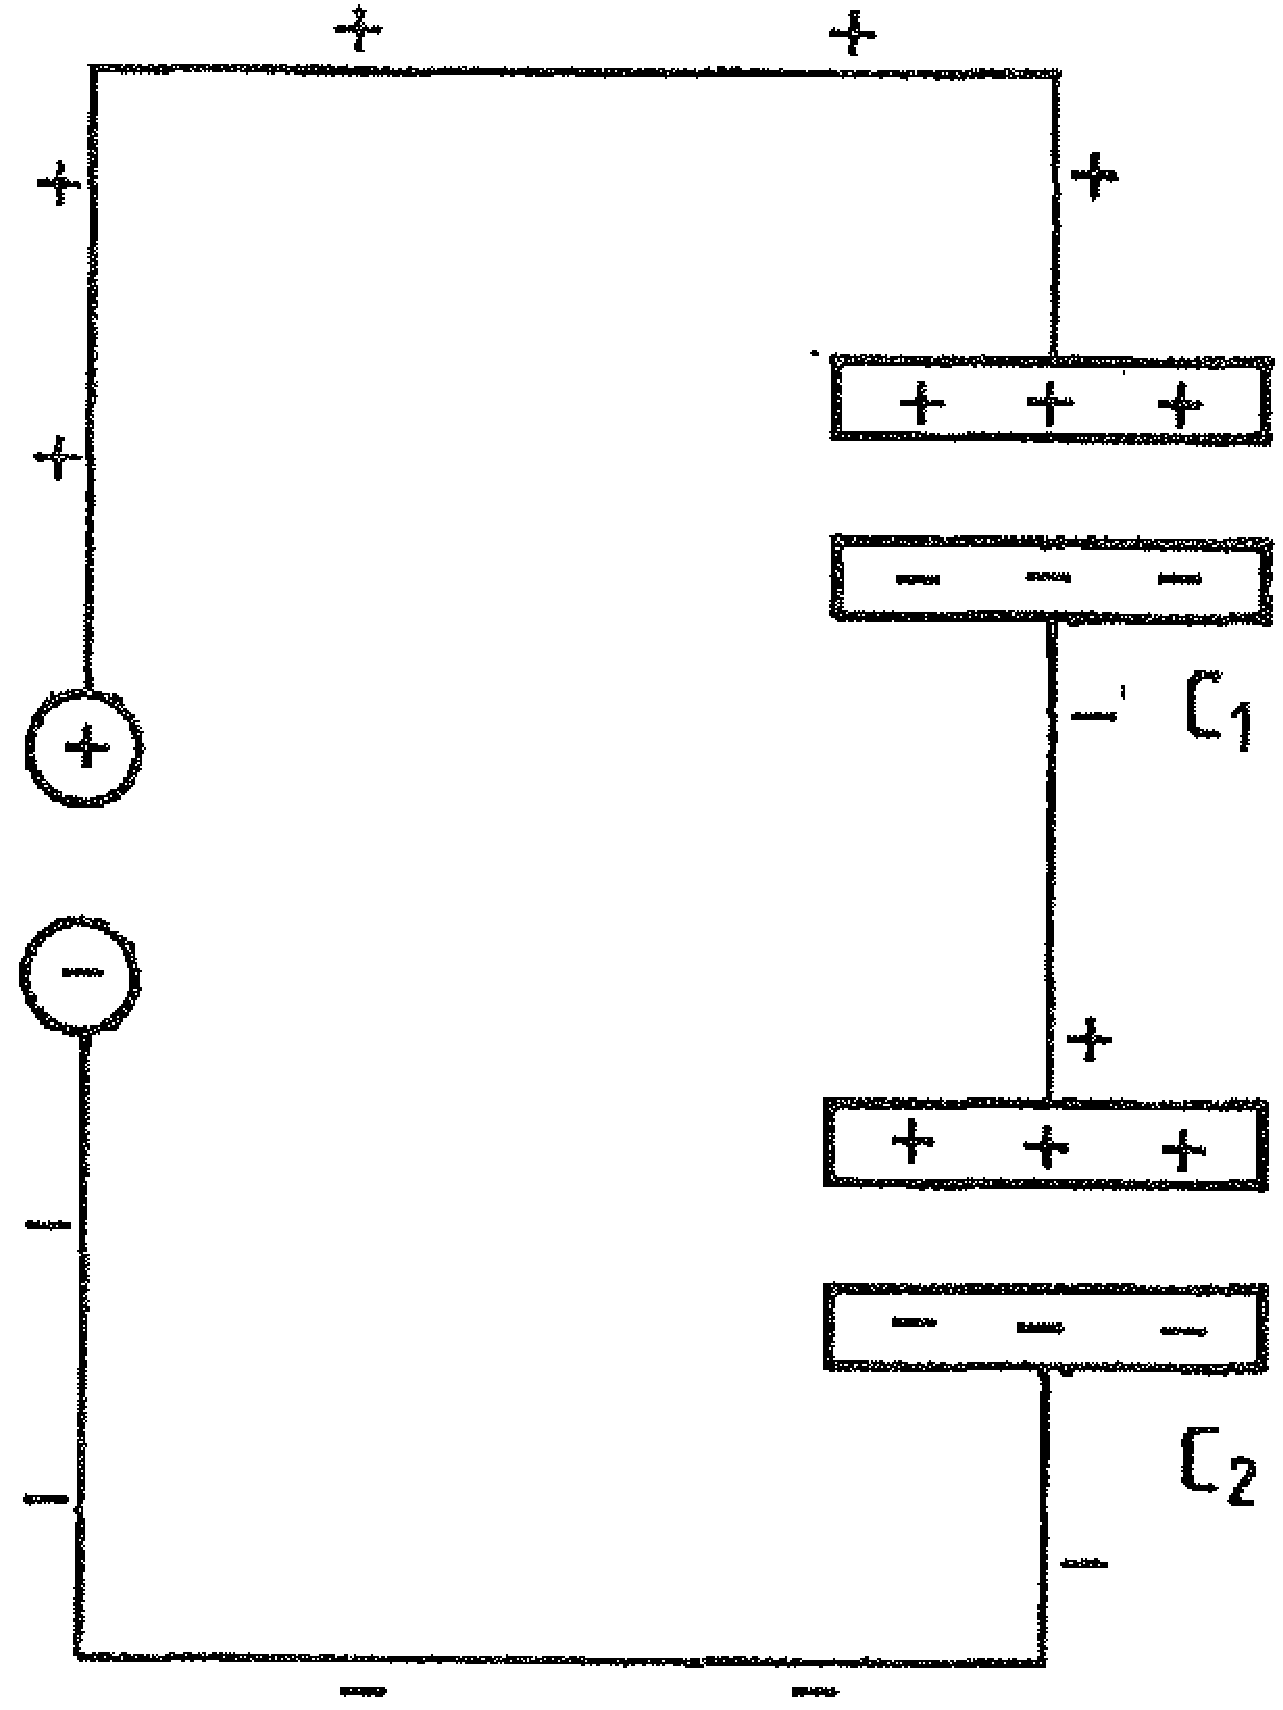
\includegraphics[width=0.5\textwidth]{images/cropped_pdfs/bild_2_3-06.pdf}
  \caption{Seriekopplade kondensatorer}
  \label{fig:BildII3-06}
  %%\end{wrapfigure}
\end{center}
\end{figure*}

Bild \ref{fig:BildII3-06} visar seriekopplade kondensatorer.
Den totala kapacitansen för seriekopplade kondensatorer är lägre än kapacitansen
för kondensatorn med det minsta värdet.

\[
\frac{1}{C} = \frac{1}{C_1} + \frac{1}{C_2} +
\frac{1}{C_3} + \cdots \frac{1}{C_n}
\]

För två kapacitanser gäller:

\begin{align*}
  \frac{1}{C} &= \frac{1}{C_1} + \frac{1}{C_2} \quad \text{eller} \\
  C &= \frac{C_1 \cdot C_2}{C_1 + C_2}
\end{align*}

För tre kapacitanser gäller:

\begin{align*}
  \frac{1}{C} &= \frac{1}{C_1} + \frac{1}{C_2} + \frac{1}{C_3}
  \quad \text{eller} \\
  C &= \frac{C_1 \cdot C_2 \cdot C_3}
  {C_1 \cdot C_2 + C_2 \cdot C_3 + C_2 \cdot C_3}
\end{align*}

\textbf{Räkneexempel:}

\begin{enumerate}
  \item \(C_1 = 5\ \mu F \quad C_2 = 10\ \mu F \quad C =\ ?\)
    \begin{align*}
      \frac{1}{C} &= \frac{1}{C_1} + \frac{1}{C_2} \\
      C &= \frac{C_1 \cdot C_2}{C_1 + C_2} \\
      &= \frac{5 \cdot 10}{5 + 10}\ \mu F \\
      &= 3\frac{1}{3}\ \mu F \\
      &\approx 3,33\ \mu F
    \end{align*}
\end{enumerate}

\subsection{Galvaniskt kopplade induktorer}

Induktansvärdet för galvaniskt sammankopplade induktorer kan i princip
beräknas på samma sätt som för motsvarande sammankoppling av resistorer.

\subsubsection{Galvaniskt seriekopplade induktorer}
\textbf{HAREC a.\ref{HAREC.a.3.1.1c}\label{myHAREC.a.3.1.1c}}
\index{induktor!seriekopplade}
\index{seriekoppling!induktorer}

Förutsatt att magnetfälten från de respektive induktorerna inte återverkar på
varandra -- det vill säga inte ''kopplar magnetiskt till varandra'' -- så
gäller:

\[L = L_1 + L_2 + L_3 + \cdots L_n\]

\textbf{Räkneexempel:}

\[L_1 = 20\ mH \quad L_2 = 50\ mH \quad L =\ ?\]
\begin{align*}
  L &= L_1 + L_2 \\
  & = 20 + 50 \\
  &= 70\ mH
\end{align*}

\subsubsection{Galvaniskt parallellkopplade induktorer}
\textbf{HAREC a.\ref{HAREC.a.3.1.1d}\label{myHAREC.a.3.1.1d}}
\index{induktor!parallellkopplade}
\index{parallellkoppling!induktorer}

Förutsatt att magnetfälten från de respektive induktorerna inte återverkar på
varandra -- det vill säga inte ''kopplar magnetiskt till varandra'' -- så
gäller:

\[
\frac{1}{L} = \frac{1}{L_1} + \frac{1}{L_2} + \frac{1}{L_3} +
\cdots \frac{1}{L_n}
\]

För två induktorer gäller:

\begin{align*}
  \frac{1}{L} &= \frac{1}{L_1} + \frac{1}{L_2} \quad \text{eller} \\
  L &= \frac{L_1 \cdot L_2}{L_1 + L_2}
\end{align*}

\textbf{Räkneexempel:}

\[L_1 = 50\ mH \quad L_2 = 60\ mH \quad L =\ ?\]
\[
  L = \frac{L_1 \cdot L_2}{L_1 + L_2} \\
  = \frac{50 \cdot 60}{50 + 60}\ mH \\
  = \frac{3000}{110}\ mH \\
  \approx 27\ mH
\]

\subsection{Magnetiskt kopplade induktorer}
\index{induktor!magnetiskt kopplade}
\index{magnetisk koppling!induktorer}
\index{ömsesidig induktans}

\begin{wrapfigure}[15]{R}{0.5\textwidth}
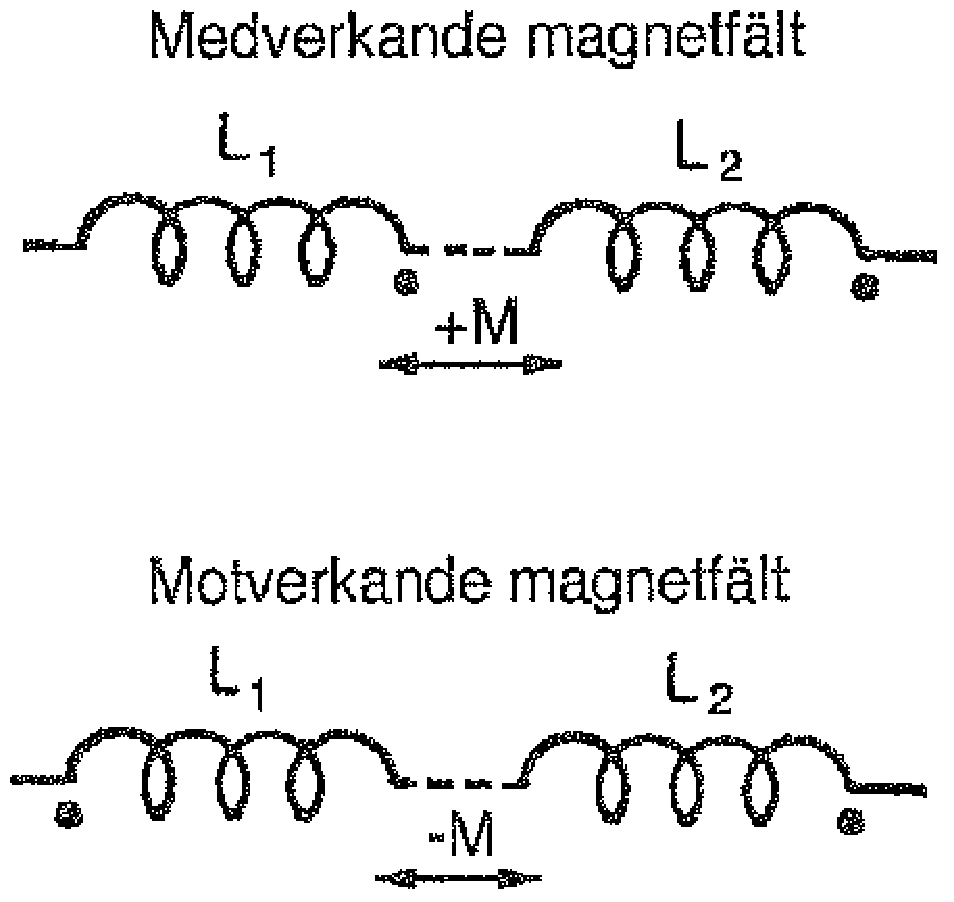
\includegraphics[width=0.5\textwidth]{images/cropped_pdfs/bild_2_3-07.pdf}
\caption{Magnetiskt kopplade induktorer}
\label{fig:BildII3-07}
\end{wrapfigure}

I praktiken anordnas ofta induktorer så, att deras respektive magnetfält kan
återverka på varandra -- så kallad magnetisk koppling.

En \emph{ömsesidig induktans} \(M\) uppstår i induktorerna på grund av denna
koppling.
Den ömsesidiga induktansen ökar eller minskar det resulterande induktansvärdet
beroende på om induktorernas magnetfält verkar med eller mot varandra.

Beräkningen av värdet på \(M\) är emellertid relativt komplicerad och behandlas
ej här.
I stället görs en förenklad framställning.

Bild \ref{fig:BildII3-07} visar seriekopplade induktorer, vars magnetfält
kopplar till varandra på olika sätt.
''Pricken'' vid änden av induktorerna på bilden markerar att magnetfälten där
har inbördes polarisering.

\subsubsection{Magnetiskt kopplade induktorer i serie}

\textbf{Formel:}

\[L = L_1 +L_2 \pm 2M\]

\textbf{Räkneexempel:}

Två induktorer har en impedans av 20 respektive 10~\(\mu H\) och en ömsesidig
induktans av 2~\(\mu H\).
Induktorerna är kopplade och placerade så att deras magnetfält verkar med
varandra.

Vardera induktansen ökas därför med \(M = 2\ \mu H\).

\begin{align*}
  L &= L_1 + M + L_2 + M \\
  &= 20 + 2 + 10 + 2\ \mu H \\
  &= 34\ \mu H
\end{align*}

\textbf{Räkneexempel:}
Två induktorer har en impedans av 20 respektive 10~\(\mu H\) och en ömsesidig
induktans av 2~\(\mu H\).
Induktorerna är kopplade och placerade så att deras magnetfält verkar mot
varandra.
Vardera induktansen minskas därför med \(M = 2\ \mu H\).

\begin{align*}
  L &= L_1 - M + L_2 - M \\
  & = 20 - 2 + 10 - 2\ \mu H \\
  &= 26\ \mu H
\end{align*}

\subsubsection{Magnetiskt kopplade induktorer i parallell}
När flera induktorer är parallellkopplade och placerade så att deras magnetiska
fält interagerar behöver man ta hänsyn till om de med- eller motverkar varandra.
Mer läsning om induktorer och hur de påverkar varandra finns att läsa i
\cite{letrafo}.

\textbf{Formler:}

Medkopplade parallella induktorer

\[L = \frac{L_1 \cdot L_2 - M^2}{L_1 + L_2 - 2M}\]

Motkopplade parallella induktorer

\[L = \frac{L_1 \cdot L_2 - M^2}{L_1 + L_2 + 2M}\]

\subsection{Upp- och urladdning av en kondensator}

\subsubsection{Uppladdning}

\begin{wrapfigure}{R}{0.5\textwidth}
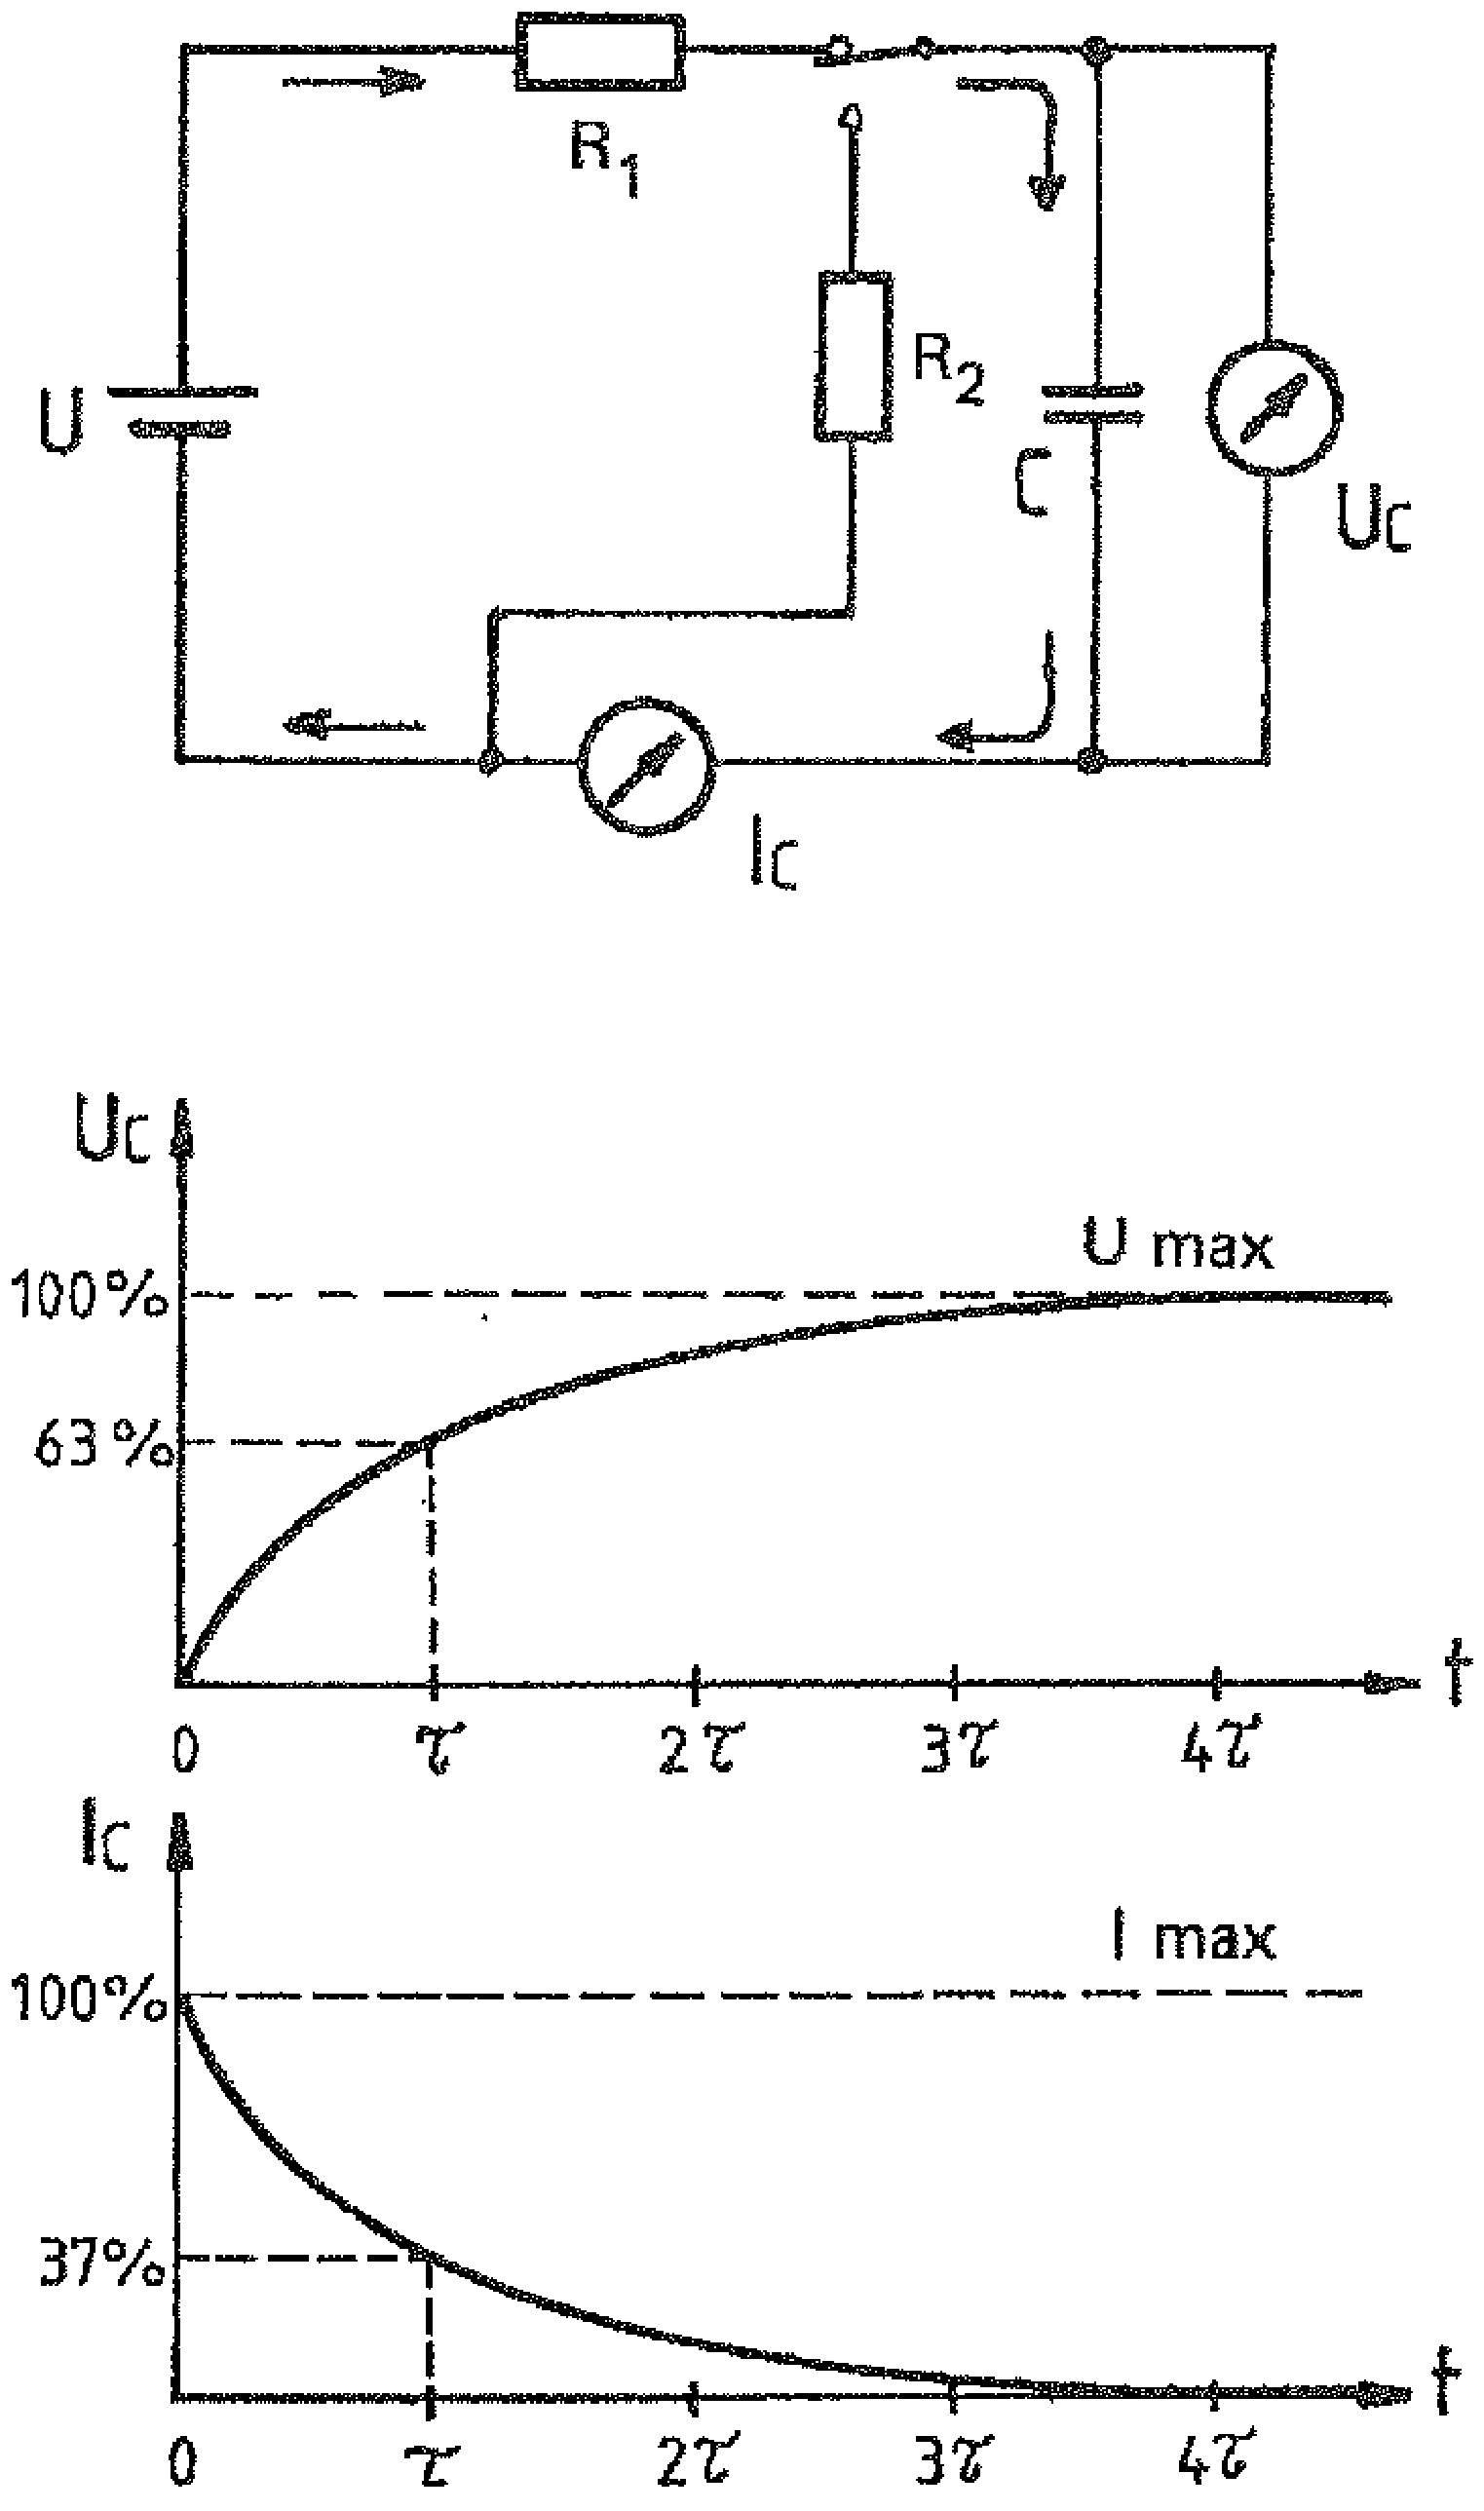
\includegraphics[width=0.5\textwidth]{images/cropped_pdfs/bild_2_3-08.pdf}
\caption{Uppladdning av en kondensator}
\label{fig:BildII3-08}
\end{wrapfigure}

Bild \ref{fig:BildII3-08} visar uppladdning av en kondensator.
En kondensator \(C\) seriekopplas med en resistans \(R\)
och kopplas in över spänningen \(U\).

Spänningen över kondensatorn stiger från 0~volt till \(U_{max}\).

Laddningsströmmen sjunker från \(I_{max}\) till 0~ampere.

Spänningen över kondensatorn ökar exponentiellt uppladdningen.

\[u_c = U_{max} \cdot ( 1 - e^{-\dfrac{t}{\tau}} )\]

\begin{tabular}{lp{0.35\textwidth}}
  \(u_c\)     & spänningen över kondensatorn efter en given inkopplingstid \\
  \(U_{max}\) & slutspänningen efter minst \(t = 5\tau\) \\
  \(t\)       & inkopplingstiden \\
  \(e\)       & 2,718 (e = basen för den naturliga logaritmen) \\
\end{tabular}

I förloppet ingår storleken av resistans och kapacitans enligt följande samband,
som kallas tidskonstant:

\begin{gather*}
  \tau = R \cdot C \\
  \tau\ [\text{tidskonstant i sek}] \\
  C\ [\text{F}] \quad R\ [\Omega]
\end{gather*}

Efter tiden \(t = 1\tau\) från inkopplingsögonblicket har spänningen över
kondensatorn ökat från noll till 63~\% av maxvärdet.
Efter tiden \(t = 5\tau\) är kondensatorn uppladdad till 99~\%.

Strömmen från kondensatorn minskar exponentiellt under uppladdningen.

\[i_c = I_{max} \cdot e^{-\dfrac{t}{\tau}}\]

\begin{tabular}{lp{0.4\textwidth}}
  \(i_c\) & strömmen från kondensatorn efter en given inkopplingstid \\
  \(I_{max}\) & begynnelseströmmen \\
\end{tabular}

Efter tiden \(t = 1\tau\) från inkopplingsögonblicket har strömmen till
kondensatorn minskat till 37~\% av maxvärdet.

Efter tiden \(t = 5\tau\) återstår 1~\% av strömmens maxvärde.

\subsubsection{Urladdning}

\begin{wrapfigure}{R}{0.5\textwidth}
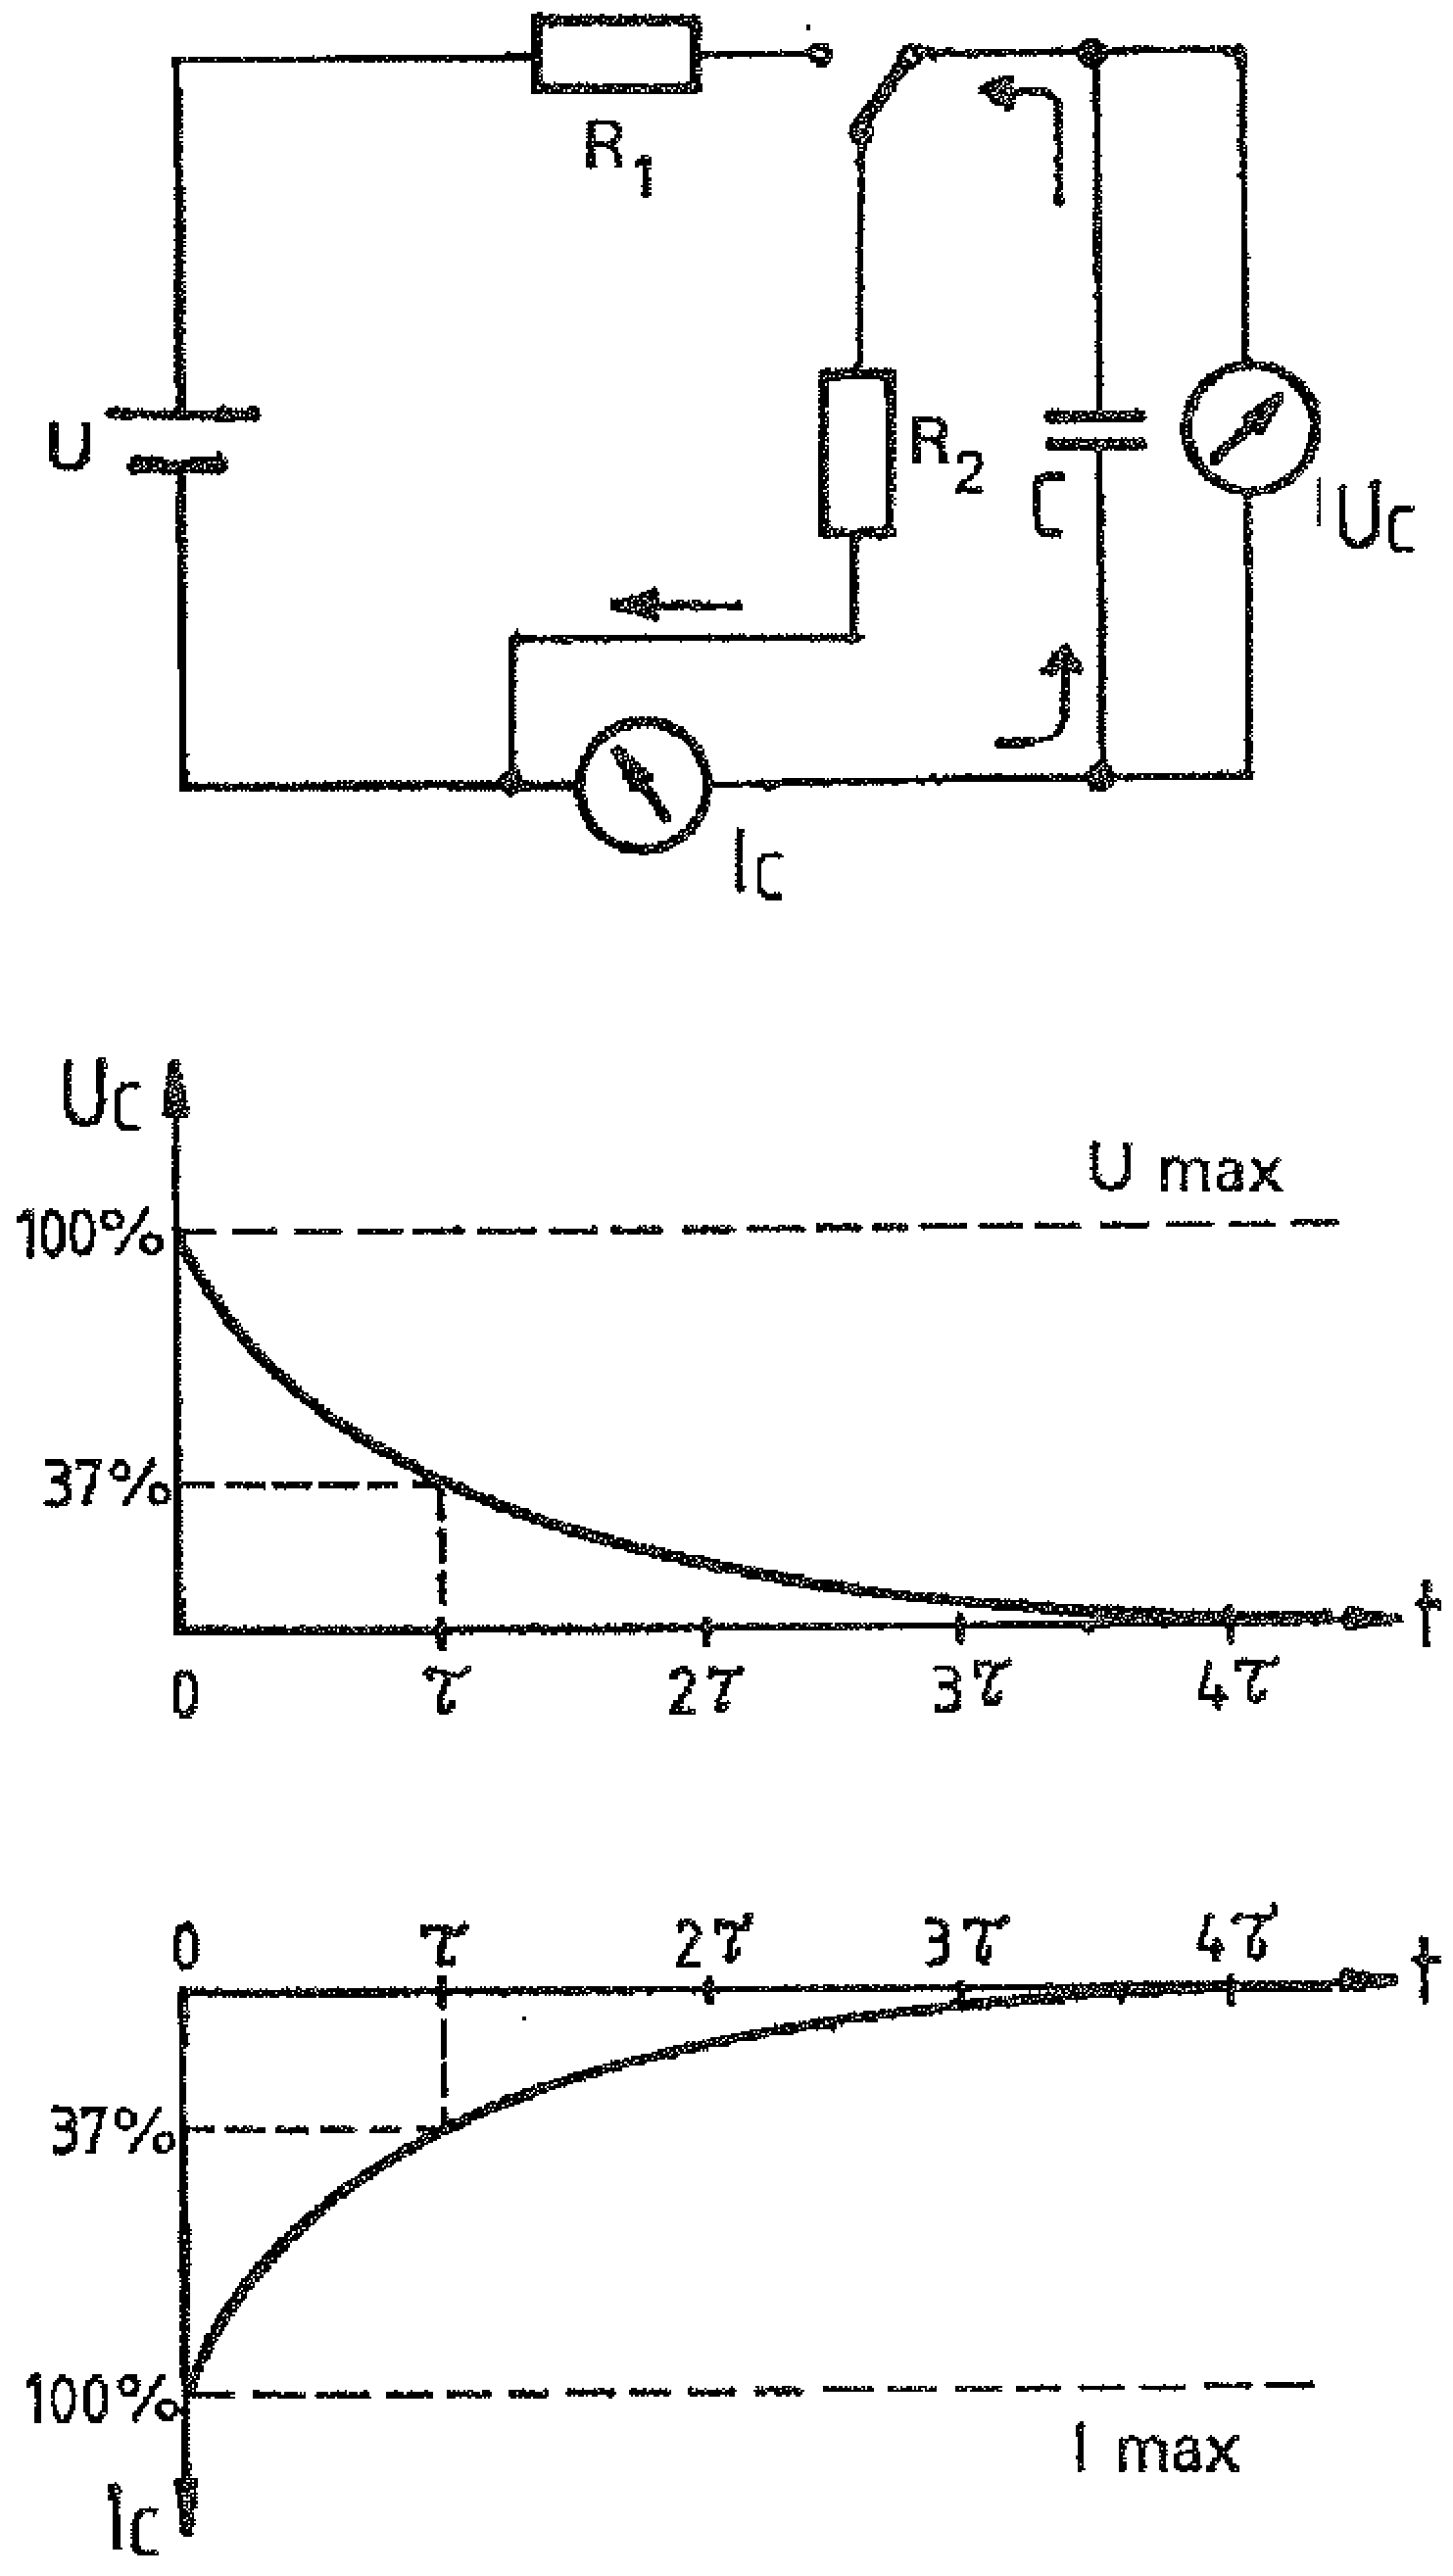
\includegraphics[width=0.5\textwidth]{images/cropped_pdfs/bild_2_3-09.pdf}
\caption{Urladdning av en kondensator}
\label{fig:BildII3-09}
\end{wrapfigure}

Bild \ref{fig:BildII3-09} visar urladdning av en kondensator.
En kondensator C urladdas över resistor R.

Spänningen över kondensatorn minskar exponentiellt under urladdningen.

\[u_c = U_{max} \cdot e^{-\dfrac{t}{\tau}}\]

Strömmen från kondensatorn minskar exponentiellt under urladdningen.
Strömriktningen är motsatt den vid uppladdningen.

\[i_c = - I_{max} \cdot e^{-\dfrac{t}{\tau}}\]

Efter tiden \(t = 1\tau\) är kondensatorn urladdad så, att 37~\% av \(I_{max}\)
respektive \(U_{max}\) återstår.

Efter tiden \(t = 5\tau\) är kondensatorn urladdad så, att mindre än 1~\% av
\(I_{max}\) respektive \(U_{max}\) återstår.

Exempel på beräkning av tidskonstanten:
\begin{enumerate}
\item \(C = 10\ \mu F \quad R = 1 k\Omega \quad \tau =\ ?\)
  \begin{align*}
    \tau &= R \cdot C \\
    &= 1 \cdot 10^3 \cdot 10 \cdot 10^{-6} \\
    &= 10 \cdot 10^{-3} \quad \text{dvs var 1/100 sekund.}
  \end{align*}
\item \(C = 1000\ \mu F \quad R = 1 k\Omega \quad \tau =\ ?\)
  \begin{align*}
    \tau &= R \cdot C \\
    &= 1 \cdot 10^3 \cdot 10^3 \cdot 10^{-6} \\
    &= 1\ \text{sekund}
  \end{align*}
\end{enumerate}

\subsection{In- och urkoppling av en induktor}

\subsubsection{Inkoppling}

\begin{wrapfigure}[23]{R}{0.5\textwidth}
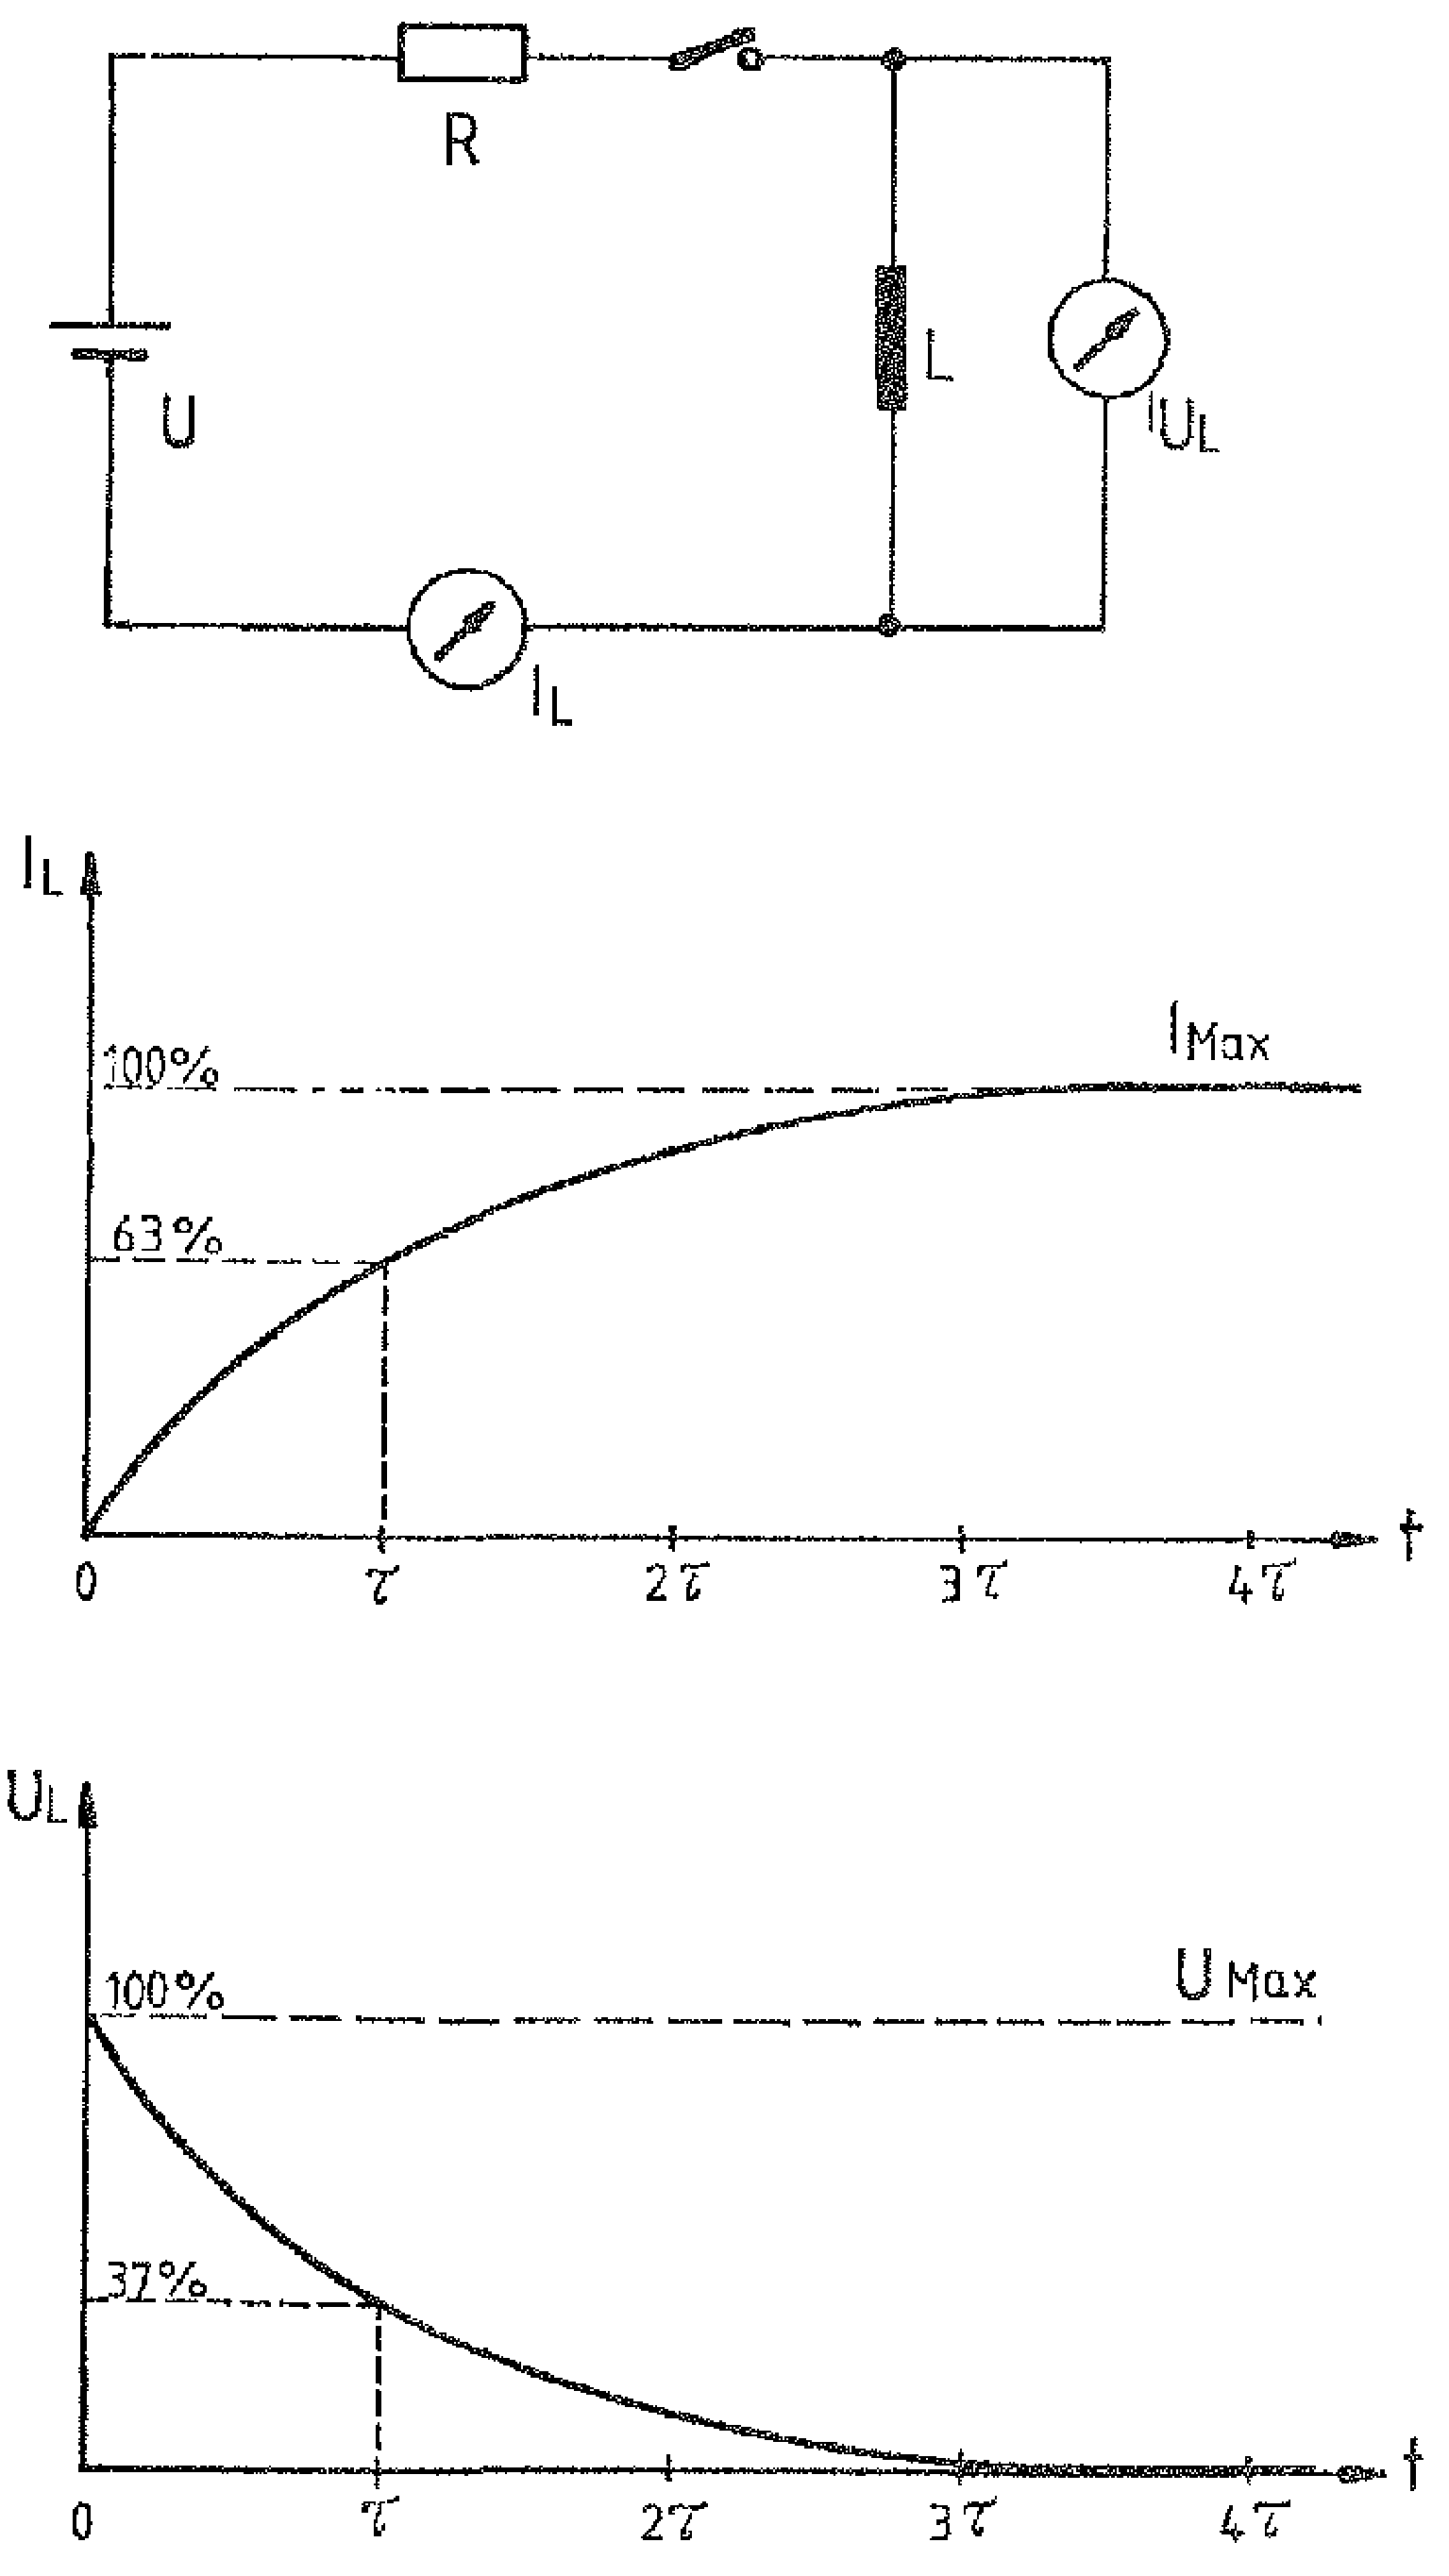
\includegraphics[width=0.5\textwidth]{images/cropped_pdfs/bild_2_3-10.pdf}
\caption{Inkoppling av en induktor}
\label{fig:BildII3-10}
\end{wrapfigure}

Bild \ref{fig:BildII3-10} visar inkopplingen av en induktor.
En induktor L i serie med en resistans R kopplas in över en likspänning U.
Spänningen över induktorn ökar från 0 till \(U_{max}\).

(Egentligen, induktorns motspänning minskar så att...)

Strömmen genom induktorn ökar från 0 till \(U_{max}\).

Strömmen genom induktorn ökar exponentiellt efter inkopplingen

\[i_L = I_{max} \cdot (1-e^{-\dfrac{t}{\tau}} )\]

\begin{tabular}{lp{0.35\textwidth}}
  \(i_L\) &  strömmen efter en given inkopplingstid \\
  \(I_{max}\) & slutströmmen efter minst \(t = 5\tau\) \\
  \(t\) & inkopplingstiden \\
  \(e\) & 2,718 (e = basen för den naturliga logaritmen) \\
\end{tabular}

I förloppet ingår storleken av resistans och induktans enligt följande samband,
som kallas tidskonstant

\[\tau = \frac{L}{R}\]

\[
L\ [\text{H}] \quad
R\ [\Omega] \quad
s\ [\text{sek}] \quad
\tau\ [\text{tidskonstant}]
\]

Efter en tid av \(t = 1\tau\) från inkopplingsögonblicket har strömmen genom
induktorn ökat från noll till 63~\% av \(I_{max}\) och motspänningen över
induktorn minskat till 37~\% av maxvärdet.

\subsubsection{Urkoppling}

Spänningskällan kopplas bort från samma induktor som ovan.
En resistor är inkopplad över induktorn.
Energin i induktorn avleds genom resistorn som en ström med motsatt riktning
än vid inkopplingen.
Strömmen är vid urkopplingstillfället \(I_{max} = i_L\) och minskar därefter
exponentiellt.

\[i_L = I_{max} \cdot e^{-\dfrac{t}{\tau}}\]

\begin{tabular}{ll}
  \(i_L\) & strömmen genom induktorn efter en given urkopplingstid \\
  \(I_{max}\) & strömmen i urkopplingsögonblicket \\
  \(e\) & 2,718 \\
  \(t\) & tiden efter urkopplingsögonblicket \\
\end{tabular}

Efter en tid av \(t = 1\tau\) från urkopplingsögonblicket har strömmen genom
induktorn minskat till 37~\% av maxvärdet.

Teoretiskt kan spänningarna och strömmarna aldrig nå ett noll- eller maxvärde,
men för praktiskt bruk anses detta inträffa efter en tid av minst \(5\tau\).

All den energi som lagras i en induktor finns i dess magnetfält.
När strömmen bryts eller minskas så återgår energin omedelbart till kretsen.
I en induktor kan det således inte finnas någon kvarstående energi, vilket
det däremot kan göra i en kondensator.

Under den tid som magnetfältet i en induktor avvecklas eller byggs upp, så
induceras en motspänning i den.
Denna spänning är högre än den som finns över induktorn innan strömmen bryts
eller ändras och är proportionell mot den hastighet som ändringen har.
När en en strömkrets med induktor bryts är det vanligt att det i
brytögonblicket bildas en gnista eller ljusbåge över brytarens kontakter.

Om induktansen är stor och kretsströmmen hög, så ska en stor mängd energi
frigöras på mycket kort tid.
Det är därför inte ovanligt att brytarkontakter bränns eller smälter.
I likströmskretsar kan gnistan eller ljusbågen minskas eller undertryckas genom
att en kondensator i serie med en resistor kopplas över kontaktstället.
Kondensatorn fångar upp en del av energin i induktorn och resistorn minskar
hastighetsändringen.

\subsection{Växelströmskretsar}
\textbf{HAREC a.\ref{HAREC.a.3.1.1}\label{myHAREC.a.3.1.1h}, a.\ref{HAREC.a.3.1.2}\label{myHAREC.a.3.1.2b}, a.\ref{HAREC.a.3.1.3}\label{myHAREC.a.3.1.3b}}

\subsubsection{Komponentegenskaper vid växelström}

Inom radiotekniken används mycket ofta svängningskretsar bestående av
kondensatorer och induktorer, som är kopplade i serie eller parallellt med
varandra.
När svängningskretsens egenfrekvens sätts lika med frekvensen på den signal som
tillförs kretsen, så får kretsen särskilda egenskaper som används på olika sätt.

För att förstå hur ''LC-kretsar'' fungerar, beskrivs först hur de ingående
komponenternas resistans, induktans och kapacitans förhåller sig till varandra,
när de kombineras och kopplas till en växelströmkälla.

\begin{figure}
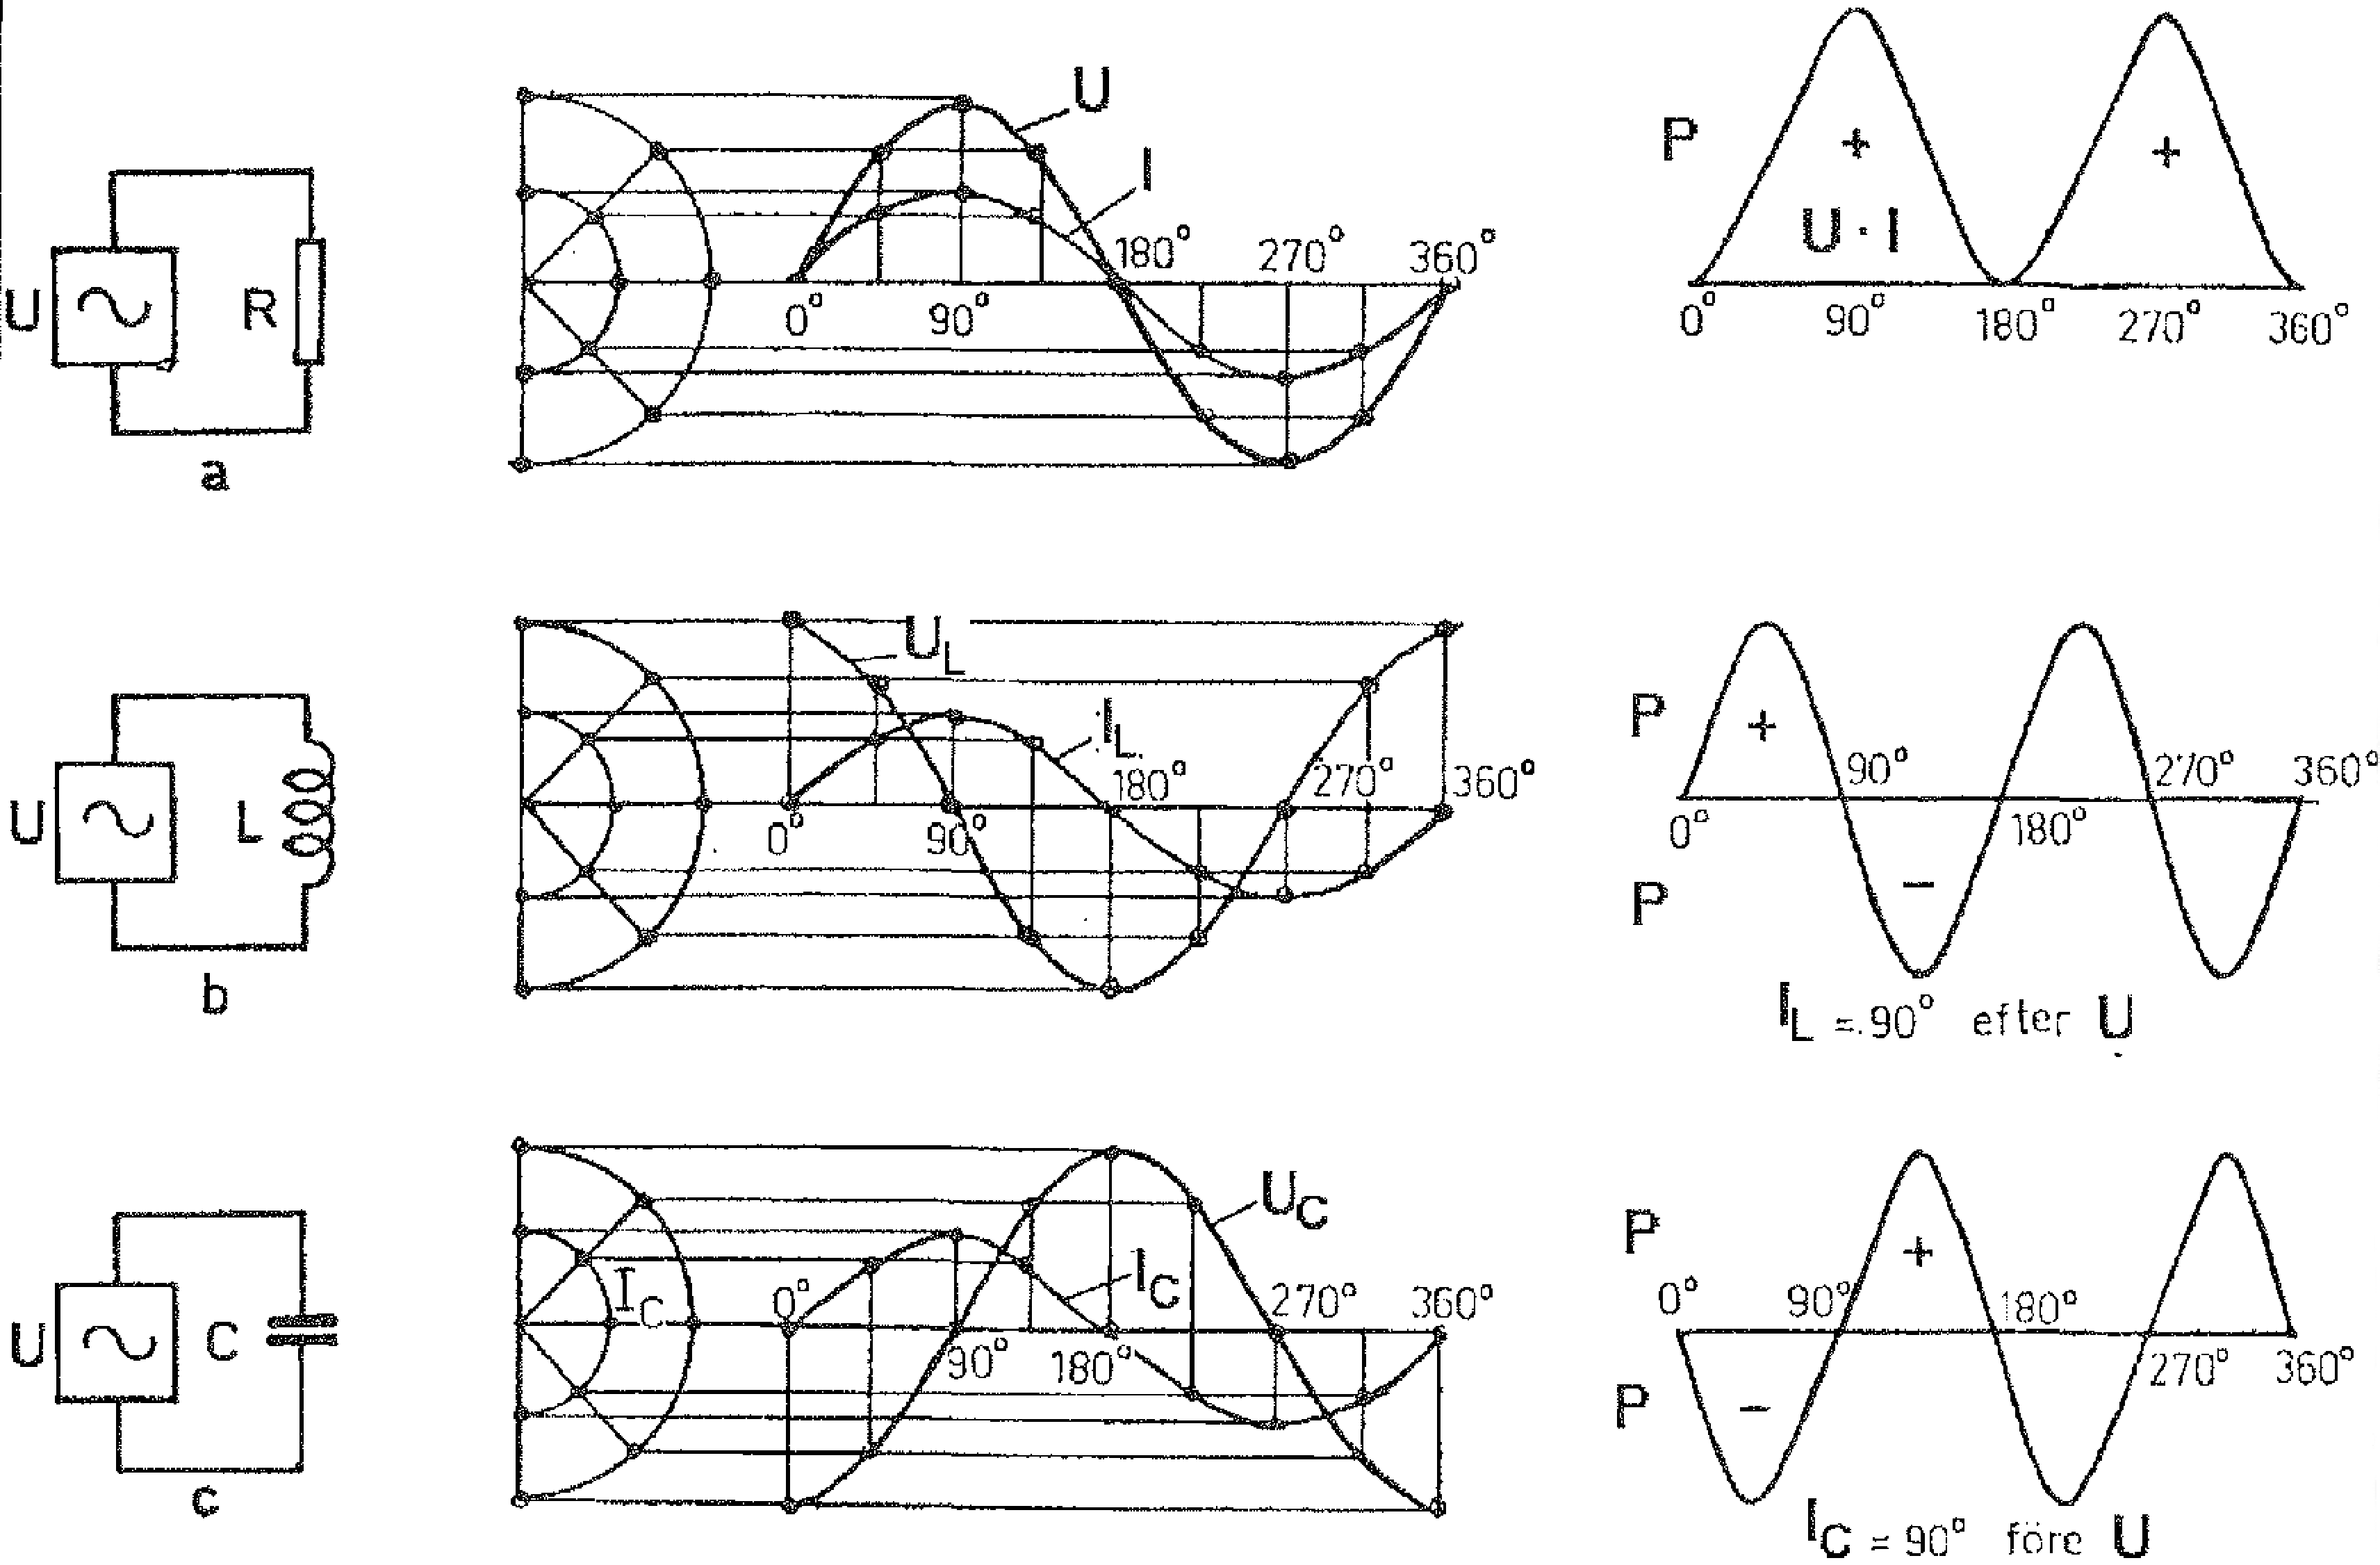
\includegraphics[width=\textwidth]{images/cropped_pdfs/bild_2_3-11.pdf}
\caption{Faslägen och effekter i L C-kretsar}
\label{fig:BildII3-11}
\end{figure}

Bild \ref{fig:BildII3-11} visar amplituden av spänning och ström vid ett
sinusformat förlopp samt den effekt som då utvecklas.
Tidsaxeln är graderad 0--360\degree~per period.

\textbf{Fall a:} Förloppen med en resistor R.

Med en resistor följer ström- och spänningskurvorna varandra tidsmässigt, även
vid riktningsändring.
När kurvorna följs åt på det sättet, sägs de vara i fas med varandra.

Effekt överförs från strömkällan till resistorn.
Den effekt som utvecklas i resistorn är, vid varje tidpunkt av perioden,
produkten av strömmen och spänningen just då.
Eftersom storheterna av spänning och ström är antingen positiva eller negativa
samtidigt, så blir produkten alltid positiv.
Det betyder att den effekt som utvecklas pulserar två gånger per period mellan
ett noll- och maxvärde.

\textbf{Fall b:} Förloppen med en induktor L.

Med en induktor är utvecklingen av ström och spänning inte samtidig.
Vid inkopplingen stiger spänningen genast till maxvärdet medan strömmen stiger
långsammare och bygger under tiden upp ett magnetfält i induktorn och omkring
övriga ledare i kretsen.

Strömmen fördröjs alltså i förhållande till spänningen.
Eftersom kurvornas max- och nollvärden inträffar vid olika tidpunkter, så heter
det att de är \emph{ur fas} eller \emph{fasförskjutna}.

En växelström genom en ideal induktor är förskjuten 90\degree~\emph{efter}
spänningen.
Strömmen når toppvärdet vid tidpunkten 90\degree~av perioden, när spänningen
nått ner till noll.
När spänningen minskar, så sjunker strömmen och tar med sig energin i
magnetfältet.
Först vid 180\degree, när spänningen har nått maxvärdet åt andra hållet, ändrar
också strömmen riktning och bygger upp ett nytt magnetfält med motsatt
polaritet.

Effekt överförs från strömkällan till induktorn när ström och spänning har
samma riktning.
När ström och spänning har olika riktning, försöker induktorn i stället
''ladda'' strömkällan med energi från sitt kraftfält.
Det pendlar därför effekt mellan strömkällan och induktorn, varvid effekten i
ena riktningen är lika stor som i andra riktningen.

Sett över en hel period upphäver därför dessa effekter varandra.
Följden blir att en ideal induktor, i motsats till en resistor, inte förbrukar
någon aktiv effekt.
Man säger att en reaktans, här en induktor, arbetar med reaktiv effekt.

I praktiken har kretsen även en viss resistans.
Därför sätts reaktansens 90\degree~fasförskjutna ström samman med resistansens
0\degree~fasförskjutna ström.
Resultatet blir en ström, som är mindre än 90\degree~ur fas, och det förbrukas
då en viss aktiv effekt i resistansen.

\textbf{Fall c:} Förloppen med en kondensator C.

Inte heller med en kondensator utvecklas ström och spänning samtidigt.
Efter inkopplingen laddar strömmen upp kondensatorn, det vill säga bygger upp
ett elektriskt fält med en viss potential (spänning).
Spänningen utvecklas långsammare än strömmen -- den blir \emph{fasförskjuten}.

Strömmen till (och från) en ideal kondensator är fasförskjuten 90\degree~före
spänningen.
När kondensatorn är kopplad till en växelströmskälla, når strömmen toppvärdet
vid tidpunkten 90\degree~eller 270\degree~av perioden.
Spänningen passerar då i båda fallen värdet noll.
När spänningen minskar, så sjunker strömmen och tar energi ur det elektriska
fältet.

Sedan strömmen passerat noll vid 180\degree~eller 0\degree/360\degree, bygger
den upp ett nytt elektriskt fält med motsatt polaritet.

Liksom med en induktor överförs effekt från strömkällan till kondensatorn när
ström och spänning har samma riktning.
När ström och spänning har olika riktning, försöker kondensatorn i stället
''ladda'' strömkällan med energi.
Det pendlar därför effekt mellan strömkällan och kondensatorn, varvid effekten i
ena riktningen är lika stor som i andra riktningen.

Sett över en hel period upphäver därför dessa effekter varandra.
Följden blir att en ideal kondensator, i motsats till en resistor, inte
förbrukar någon aktiv effekt.
Man säger då, att en reaktans, här en kondensator, arbetar med \emph{reaktiv}
effekt.

I praktiken har kretsen även en viss resistans.
Därför sätts reaktansens 90\degree~fasförskjutna spänning samman med
resistansens 0\degree~fasförskjutna ström.
Resultatet blir en spänning, som är mindre än 90\degree~ur fas, och det
förbrukas då en viss aktiv effekt i resistansen.
Som framgår av bilden blir variationerna i tiden de omvända med kondensator
jämfört med induktor.

\subsection{Impedans}
\textbf{HAREC
  a.\ref{HAREC.a.3.1.3}\label{myHAREC.a.3.1.3c},
  a.\ref{HAREC.a.3.2.2}\label{myHAREC.a.3.2.2}
}
\index{impedans}
\index{resistans}
\index{reaktans}

Liten ordlista:
\begin{itemize}
\item Impedans -- hindra (lat. impedire).
\item Resistans -- motstå (lat. resistere).
  Del av impedansen, kallas ibland ohmskt motstånd.
\item Reaktans- återverka (lat. reagere).
  Del av impedansen, samlingsord för växelströmsmotstånd.
  \begin{itemize}
  \item Kapacitans -- inrymma (lat. capax). Del av reaktansen.
  \item Induktans -- införa (lat. inducere). Del av reaktansen.
  \end{itemize}
\end{itemize}

Hittills har storheterna resistans, induktans och kapacitans behandlats var för
sig, men i praktiken förekommer de alltid tillsammans och kallas impedans.

Resistansen är i princip oförändrad vid ström- eller spänningsändringar.
Men när strömmen genom en ledare eller induktor liksom spänningen över en
kondensator ändras, så tillkommer en reaktans som motverkar förändringarna.

Reaktansen kan från fall till fall vara kapacitiv eller induktiv och ingår i
impedansen.
Om ingen reaktans finns, så är impedansen lika med resistansen.

\begin{wrapfigure}{R}{0.5\textwidth}
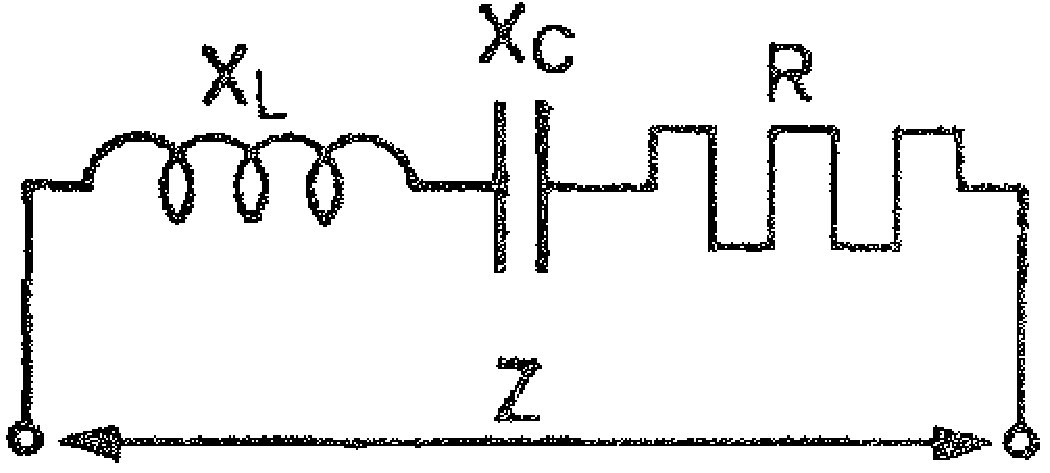
\includegraphics[width=0.5\textwidth]{images/cropped_pdfs/bild_2_3-12.pdf}
\caption{Seriekrets av L+C+R}
\label{fig:BildII3-12}
\end{wrapfigure}

Bild \ref{fig:BildII3-12} visar en induktor, en kondensator och en resistor
som är kopplade i serie.
När man vill beräkna den resulterande impedansen i kretsen
(''totala växelströmsmotståndet''), måste man ta hänsyn till att komponenternas
spänningar eller strömmar inte är i fas med varandra.
De arbetar ju inte ''i takt''.

Att då addera maxvärdena ger fel resultat.
I stället söker man den så kallade resultanten av de olika vektorer som
motsvarar ström- och spänningsvärden.
Detta kan göras grafiskt eller beräknas.

\begin{figure}
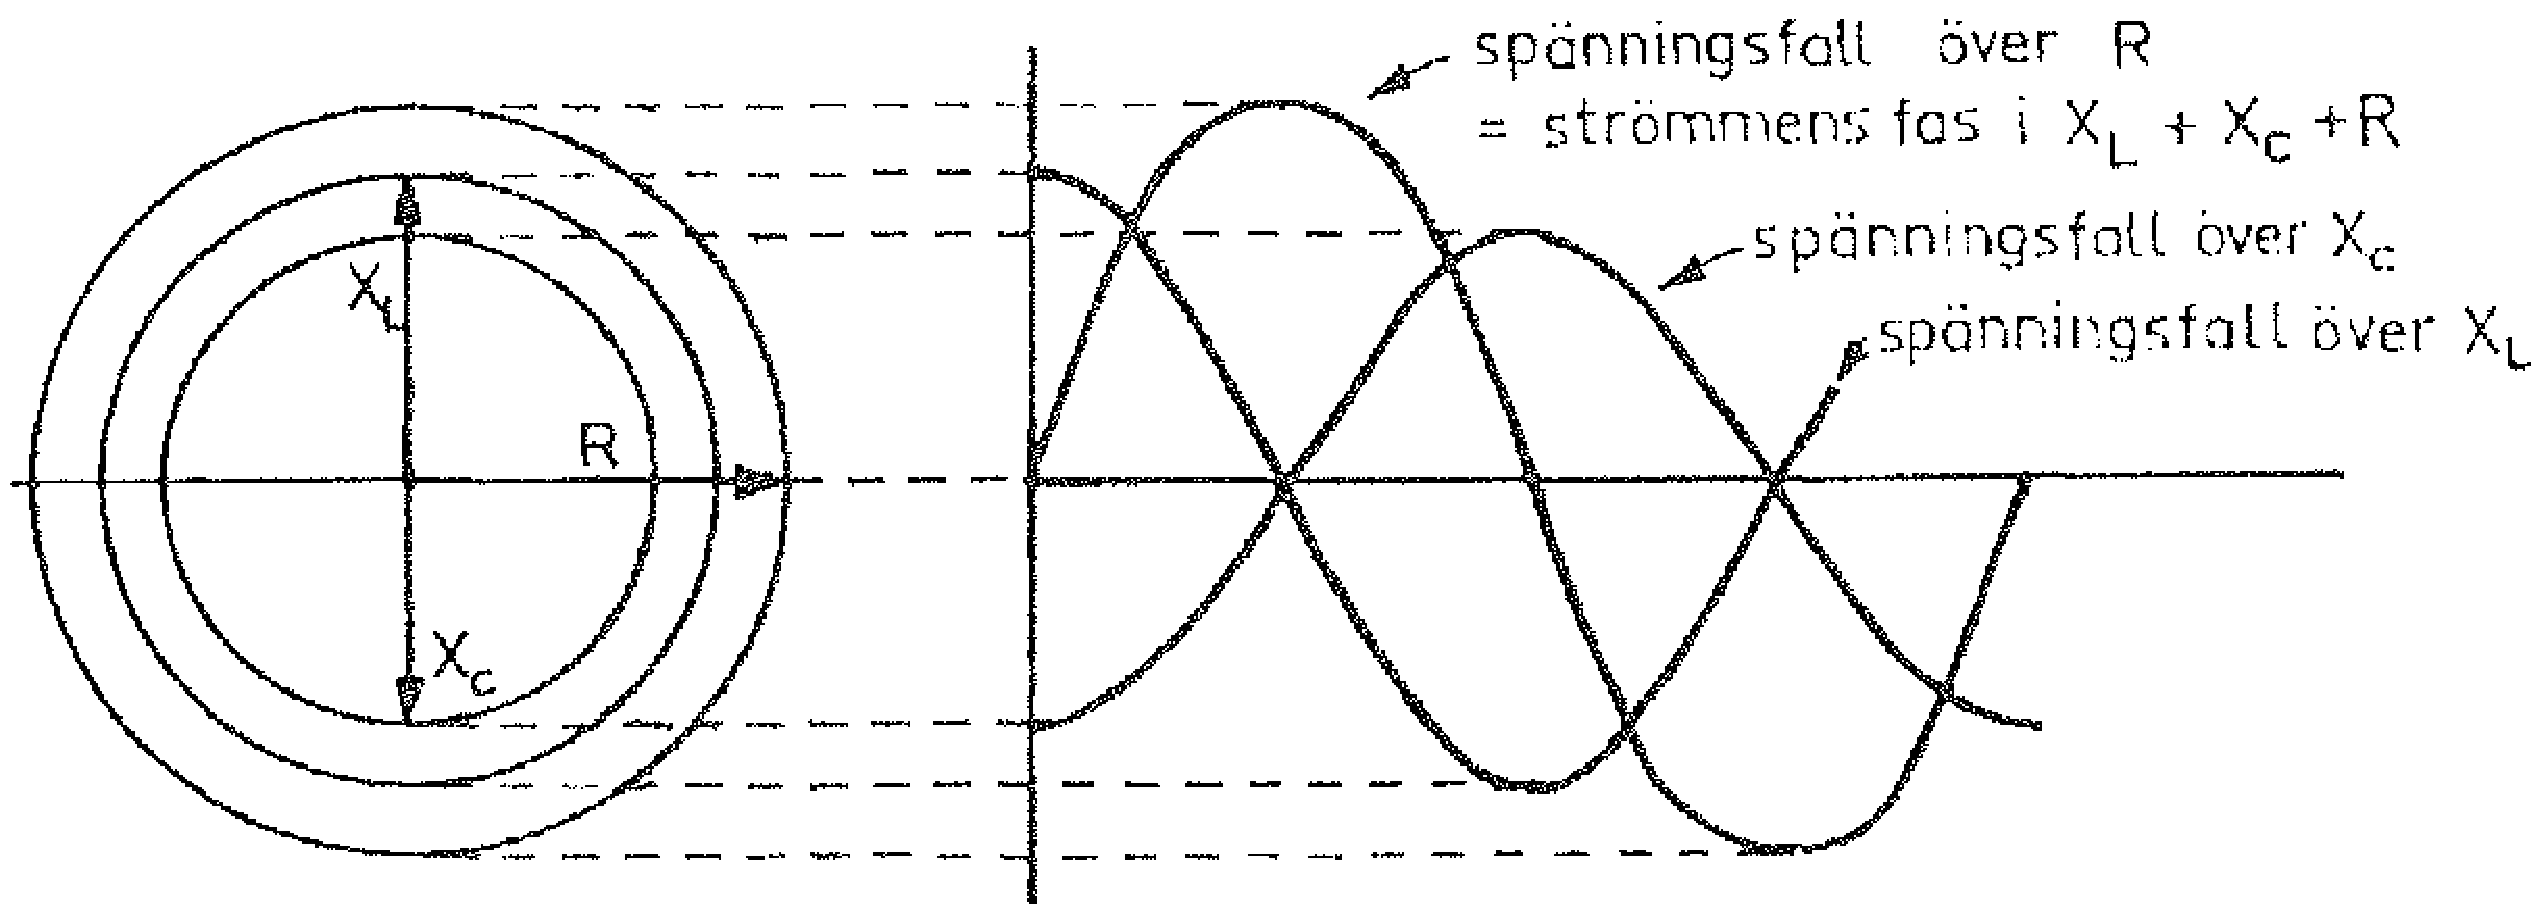
\includegraphics[width=\textwidth]{images/cropped_pdfs/bild_2_3-13.pdf}
\caption{Spänningar i seriekrets L+C+R}
\label{fig:BildII3-13}
\end{figure}

Bild \ref{fig:BildII3-13}

Vi tänker oss att vektorerna i systemet vrider sig moturs med hastigheten
\(\omega = 2\pi f\) där \(f\) är frekvensen och \(\omega\) är vinkelhastighet.
Eftersom vektorerna har samma frekvens, så är vektorernas lägen inbördes samma.
Ögonblicksvärdet av respektive vektorer följer en sinuskurva.

Spänningsvektorn i den ''induktiva reaktansen'' ligger 90\degree~före strömmen
och spänningen i resistansen.
Spänningsvektorn i den ''kapacitiva reaktansen'' ligger 90\degree~efter
strömmen och spänningen i resistansen.
Vektorerna i dessa två reaktanser är således \(2 \cdot 90 = 180\degree\)
åtskilda, det vill säga motriktade.
Det kallas att de är i motfas.

\begin{figure}
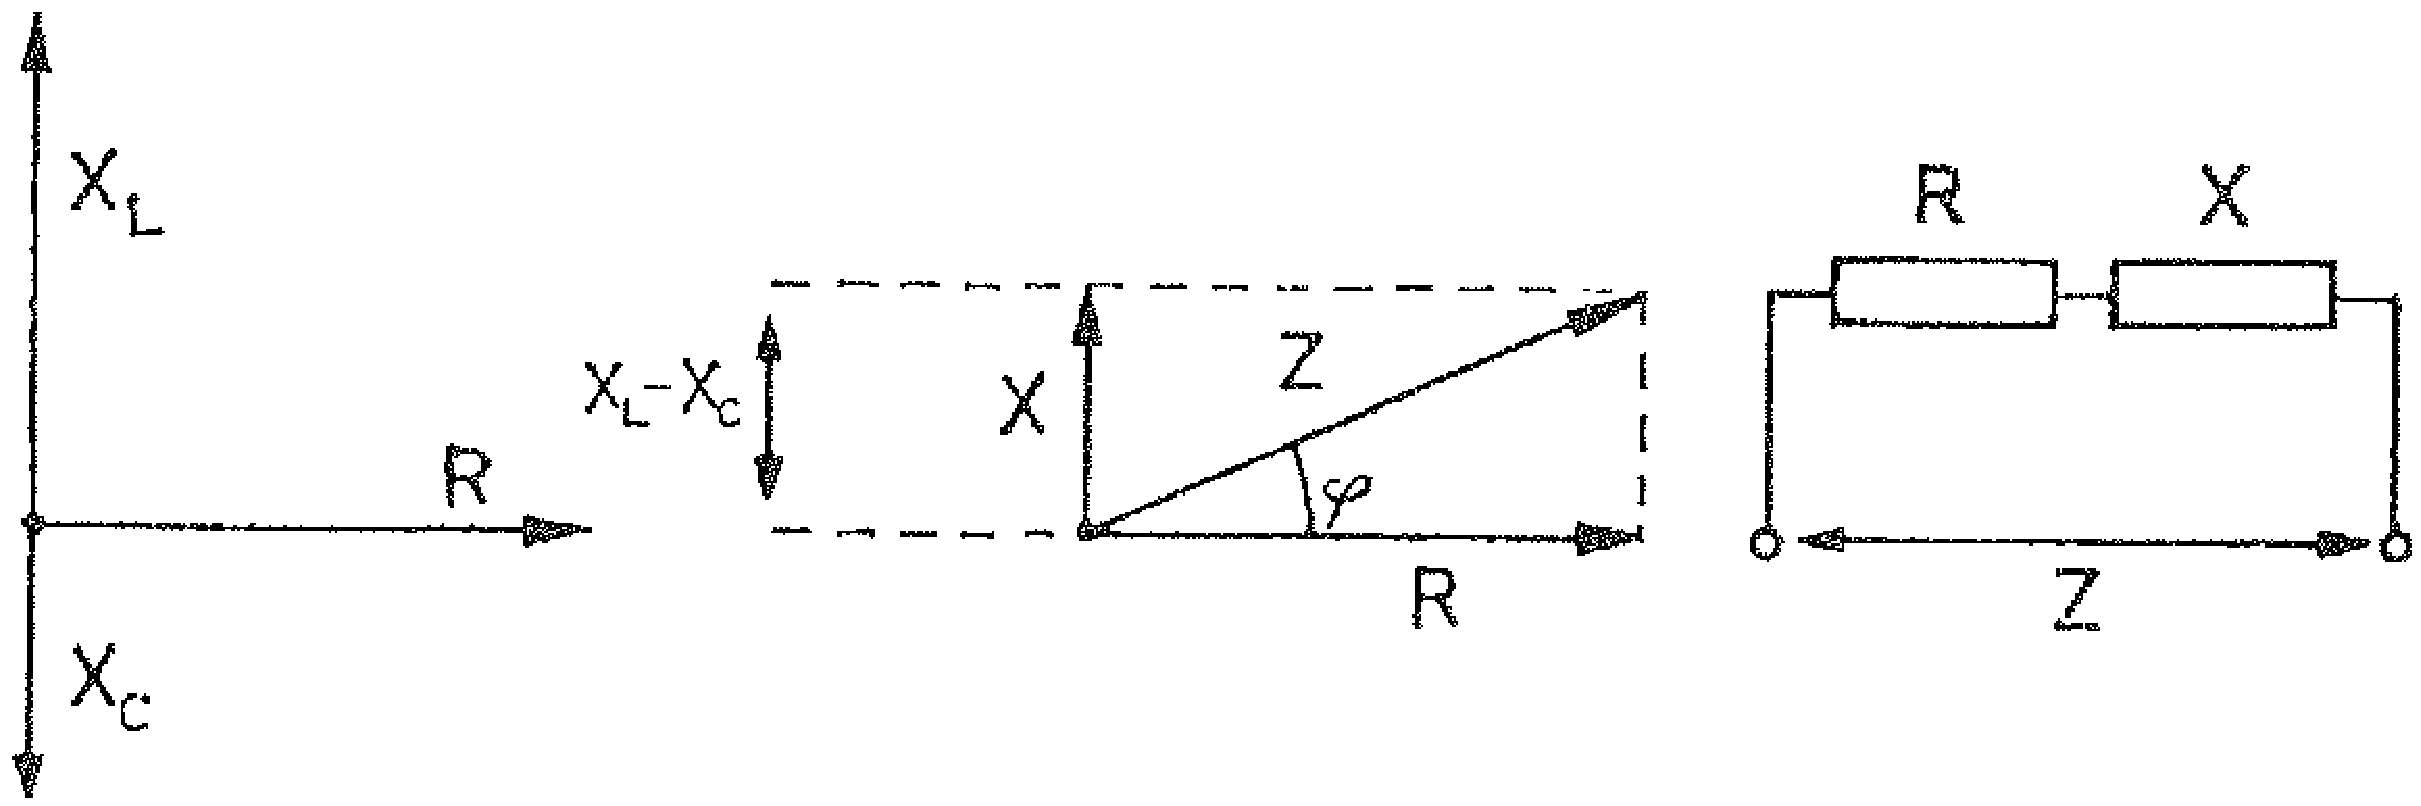
\includegraphics[width=\textwidth]{images/cropped_pdfs/bild_2_3-14.pdf}
\caption{Impedansen och fasvinkeln i seriekrets L+C+R}
\label{fig:BildII3-14}
\end{figure}

I bild \ref{fig:BildII3-14} visas vektorerna för komponenterna i bild
\ref{fig:BildII3-12} samt hur man grafiskt bestämmer impedansen av dessa
vektorer.
Vidare får man fasvinkeln mellan impedansens och resistansens vektor, varav den
senare är den så kallade riktfasen för hela seriekretsen.

Resistansen ritas som en vektor \(R\), som riktas vågrätt mot höger.
Vektorns längd motsvarar resistansens storlek i ohm.

Den induktiva reaktansen ritas på liknande sätt med vektorn \(X_L\) lodrätt
uppåt.
Slutligen ritas den kapacitiva reaktansen \(X_C\) lodrätt neråt.

Man subtraherar de motverkande reaktiva vektorerna \(X_L\) och \(X_c\) från
varandra och avsätter resultatet \(X\) på den vertikala axeln, uppåt om \(X_L\)
är större och neråt om \(X_c\) är större.
Den resistiva vektorn \(R\) avsätts åt höger på den horisontella axeln.

Man låter nu vektorerna \(X\) och \(R\) bilda sidor i en rätvinklig rektangel.
Längden på rektangelns diagonal är den resulterande impedansen \(Z\).
Fasvinkeln mellan impedans och resistans kan också avläsas.

Eftersom vektordiagrammet bildar en rätvinklig triangel kan den resulterande
spänningen \(U\) i kretsen även beräknas med Pytagoras sats:

\[C^2 = A^2 + B^2 \quad eller \quad C = \sqrt{A^2 + B^2}\]

Tillämpad på ovanstående vektordiagram kan satsen skrivas som

\[U_{LCR}^2 = U_R^2 + ( U_L - U_C)^2\]

Termerna ersätts med följande ekvationer:

\begin{align*}
  U_{LRC} &= I \cdot Z \\
  U_R &= I \cdot R \\
  U_L &= I X_L = I \omega L \\
  U_C &= I X_C = I \frac{1}{\omega C} \\
  I^2 Z^2 &= I^2 R^2 + ( I \omega L - I\frac{1}{\omega C})^2
\end{align*}

Efter division med \(I^2\) fås

\begin{align*}
  Z^2 &= R^2 + ( \omega L - \frac{1}{\omega C} )^2 \quad \text{eller} \\
  Z &= \sqrt{R^2 + (\omega L - \frac{1}{\omega C})^2} \quad \text{eller} \\
  Z &= \sqrt{R^2 + (X_L - X_C)^2}
\end{align*}

I en seriekrets är den resulterande reaktansen negativ (kapacitiv) om \(X_C\) är
större än \(X_L\) och positiv (induktiv) om \(X_L\) är större än \(X_C\).

\subsection{Ohms lag vid växelström}
\textbf{HAREC
  a.\ref{HAREC.a.1.1.4}\label{myHAREC.a.1.1.4b}
}

I formler betecknas impedansen med bokstaven \(Z\) och reaktansen med bokstaven
\(X\).
I båda fallen är enheten ohm [\(\Omega\)].

Vid beräkning av impedans är Ohms lag inte direkt tillämplig, eftersom
reaktansen i en induktor eller kondensator uppträder annorlunda i tiden vid
ström- respektive spänningsändring än vad resistansen gör.

Om impedansen \(Z\) sätts in i Ohms lag, så fås följande samband som ofta kallas
Ohms lag för växelström, således

\begin{align*}
  U_{eff} &= I_{eff} \cdot Z \quad \text{eller} \\
  U_{eff} &= I_{eff} \cdot \sqrt{R^2 + X^2} \quad \text{eller} \\
  U_{eff} &= I_{eff} \cdot \sqrt{R^2 + (X_L - X_C)^2} \quad \text{osv.}
\end{align*}

Av vad som framgått tidigare i detta avsnitt kan även slutsatsen dras att:

\[
\text{skenbar effekt} = \sqrt{(\text{aktiv effekt})^2 + (\text{reaktiv effekt})^2}
\]

\subsection{LC-kretsar}
\textbf{HAREC
  a.\ref{HAREC.a.3.1.3}\label{myHAREC.a.3.1.3d},
  a.\ref{HAREC.a.3.2.1}\label{myHAREC.a.3.2.1}
}
\index{LC-krets}

\subsubsection{Parallellkopplade LC-kretsar}
\index{parallellkopplad LC-krets}
\index{LC-krets!parallellkopplad}

\begin{figure}
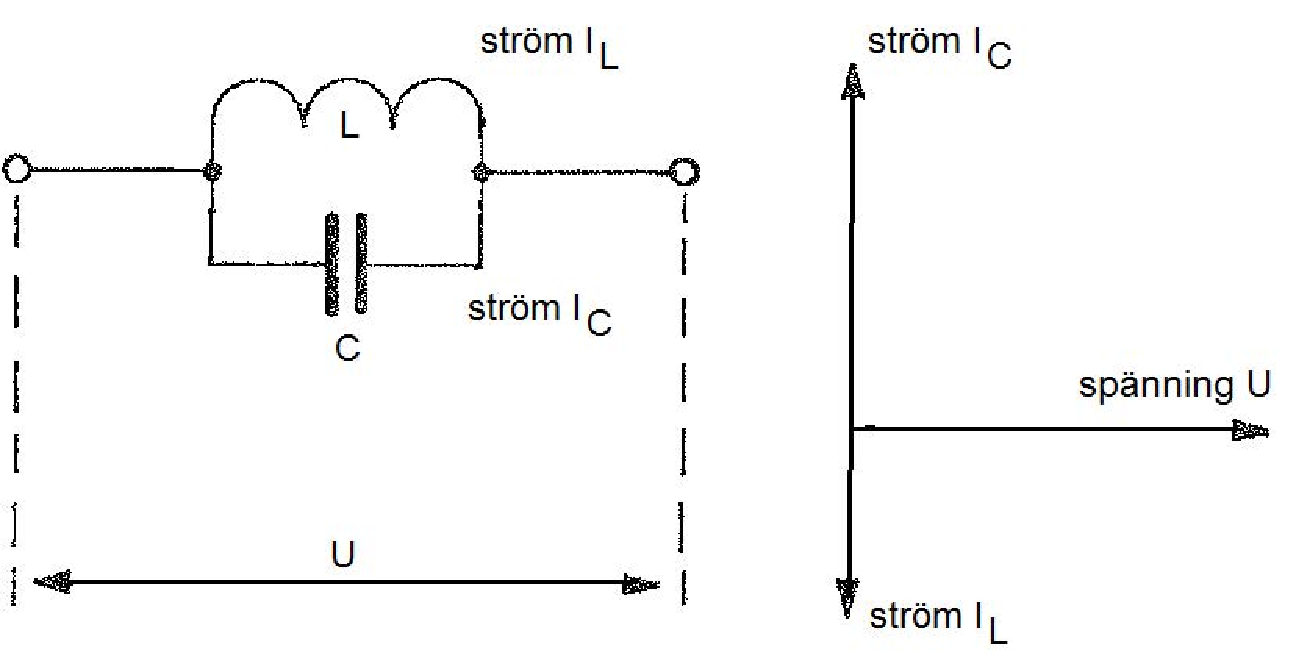
\includegraphics[width=\textwidth]{images/cropped_pdfs/bild_2_3-15.pdf}
\caption{Parallellkopplad LC-krets}
\label{fig:BildII3-15}
\end{figure}

En parallellkopplad LC-krets är i bild \ref{fig:BildII3-15} ansluten till
växelspänningen \(U\) från en signalgenerator med inställbar frekvens \(f\).
Två fall studeras.

\textbf{Fall 1:} \(f = f_{res}\)

Signalgeneratorns frekvens \(f\) ställs lika med LC-kretsens resonansfrekvens
\(f_{res}\).
Då visar kretsen hög impedans \(Z\) mot generatorn.
En stark ström cirkulerar i svängningskretsen, men endast en svag ström flyter
i ledningen mellan generator och krets.
Jämför med modellförsöket på bild \ref{fig:BildII3-17}.

\textbf{Fall 2:} \(f > f_{res}\) eller \(f < f_{res}\)

Frekvensen \(f\) ställs högre eller lägre än kretsens resonansfrekvens
\(f_{res}\).

Svängningskretsen visar då en låg impedans \(Z\) mot generatorn.
En svag ström cirkulerar i svängningskretsen, medan en starkare ström flyter i
ledningen mellan generator och krets.

I praktiken finns även en resistans (belastning) parallellt över kretsen och en
resistans i serie med induktansen.
För enkelhetens skull bortses här från dessa resistanser.

I en parallellkopplad LC-krets är spänningen över induktans och kapacitans
densamma.
Spänningsvektorn \(U\) används därför som så kallad riktfas.

Riktfasen ritas på bilden åt höger.
Strömmen \(I_C\) genom kondensatorn är fasförskjuten 90\degree~efter \(U\) och
ritas rakt neråt (vektorerna roterar motsols).
Strömmen \(I_L\) genom induktorn är fasförskjuten 90\degree~före \(U\) och
ritas rakt uppåt.
Den resulterande reaktiva strömmen genom kretsen är skillnaden mellan
strömmarna \(I_C\) och \(I_L\), vilka är motriktade varandra.

Formeln för parallellkopplade resistanser kan även användas för
parallellkopplade reaktanser om man tillämpar Pytagoras sats
\(A^2 + B^2 = C^2\), således

\begin{gather*}
  \frac{1}{R} = \frac{1}{R_1} + \frac{1}{R_1} + \cdots \\
  \left(\frac{1}{Z}\right)^2 = \left(\frac{1}{R}\right)^2 +
  \left(\frac{1}{R}\right)^2 \quad \text{eller}
\end{gather*}
\begin{align*}
  \frac{1}{Z} &=
  \sqrt{\left(\frac{1}{R}\right)^2 + \left(\frac{1}{X}\right)^2} \\
  &= \sqrt{\frac{1}{R^2} + \frac{1}{X^2}}
\end{align*}

Med \(R\) försumbart kan den resulterande reaktansen av kapacitansen \(X_C\)
och den vektormässigt motriktade induktansen \(X_L\) beräknas på följande sätt:

\begin{align*}
  \frac{1}{X} &= \frac{1}{X_C} - \frac{1}{X_L} \quad \text{dvs.} \quad
  \frac{1}{X} = \frac{X_L - X_C}{-X_L \cdot X_C} \quad \text{eller} \\
  X &= \frac{-X_L \cdot X_C}{X_L - X_C}
\end{align*}

I en parallellkopplad LC-krets är den resulterande reaktansen negativ
(kapacitiv) om \(X_L\) är större än \(X_C\) och positiv (induktiv) om \(X_L\) är
mindre än \(X_C\).

\subsection{Seriekopplade LC-kretsar}
\index{seriekopplad LC-krets}
\index{LC-krets!seriekopplad}

\begin{figure}
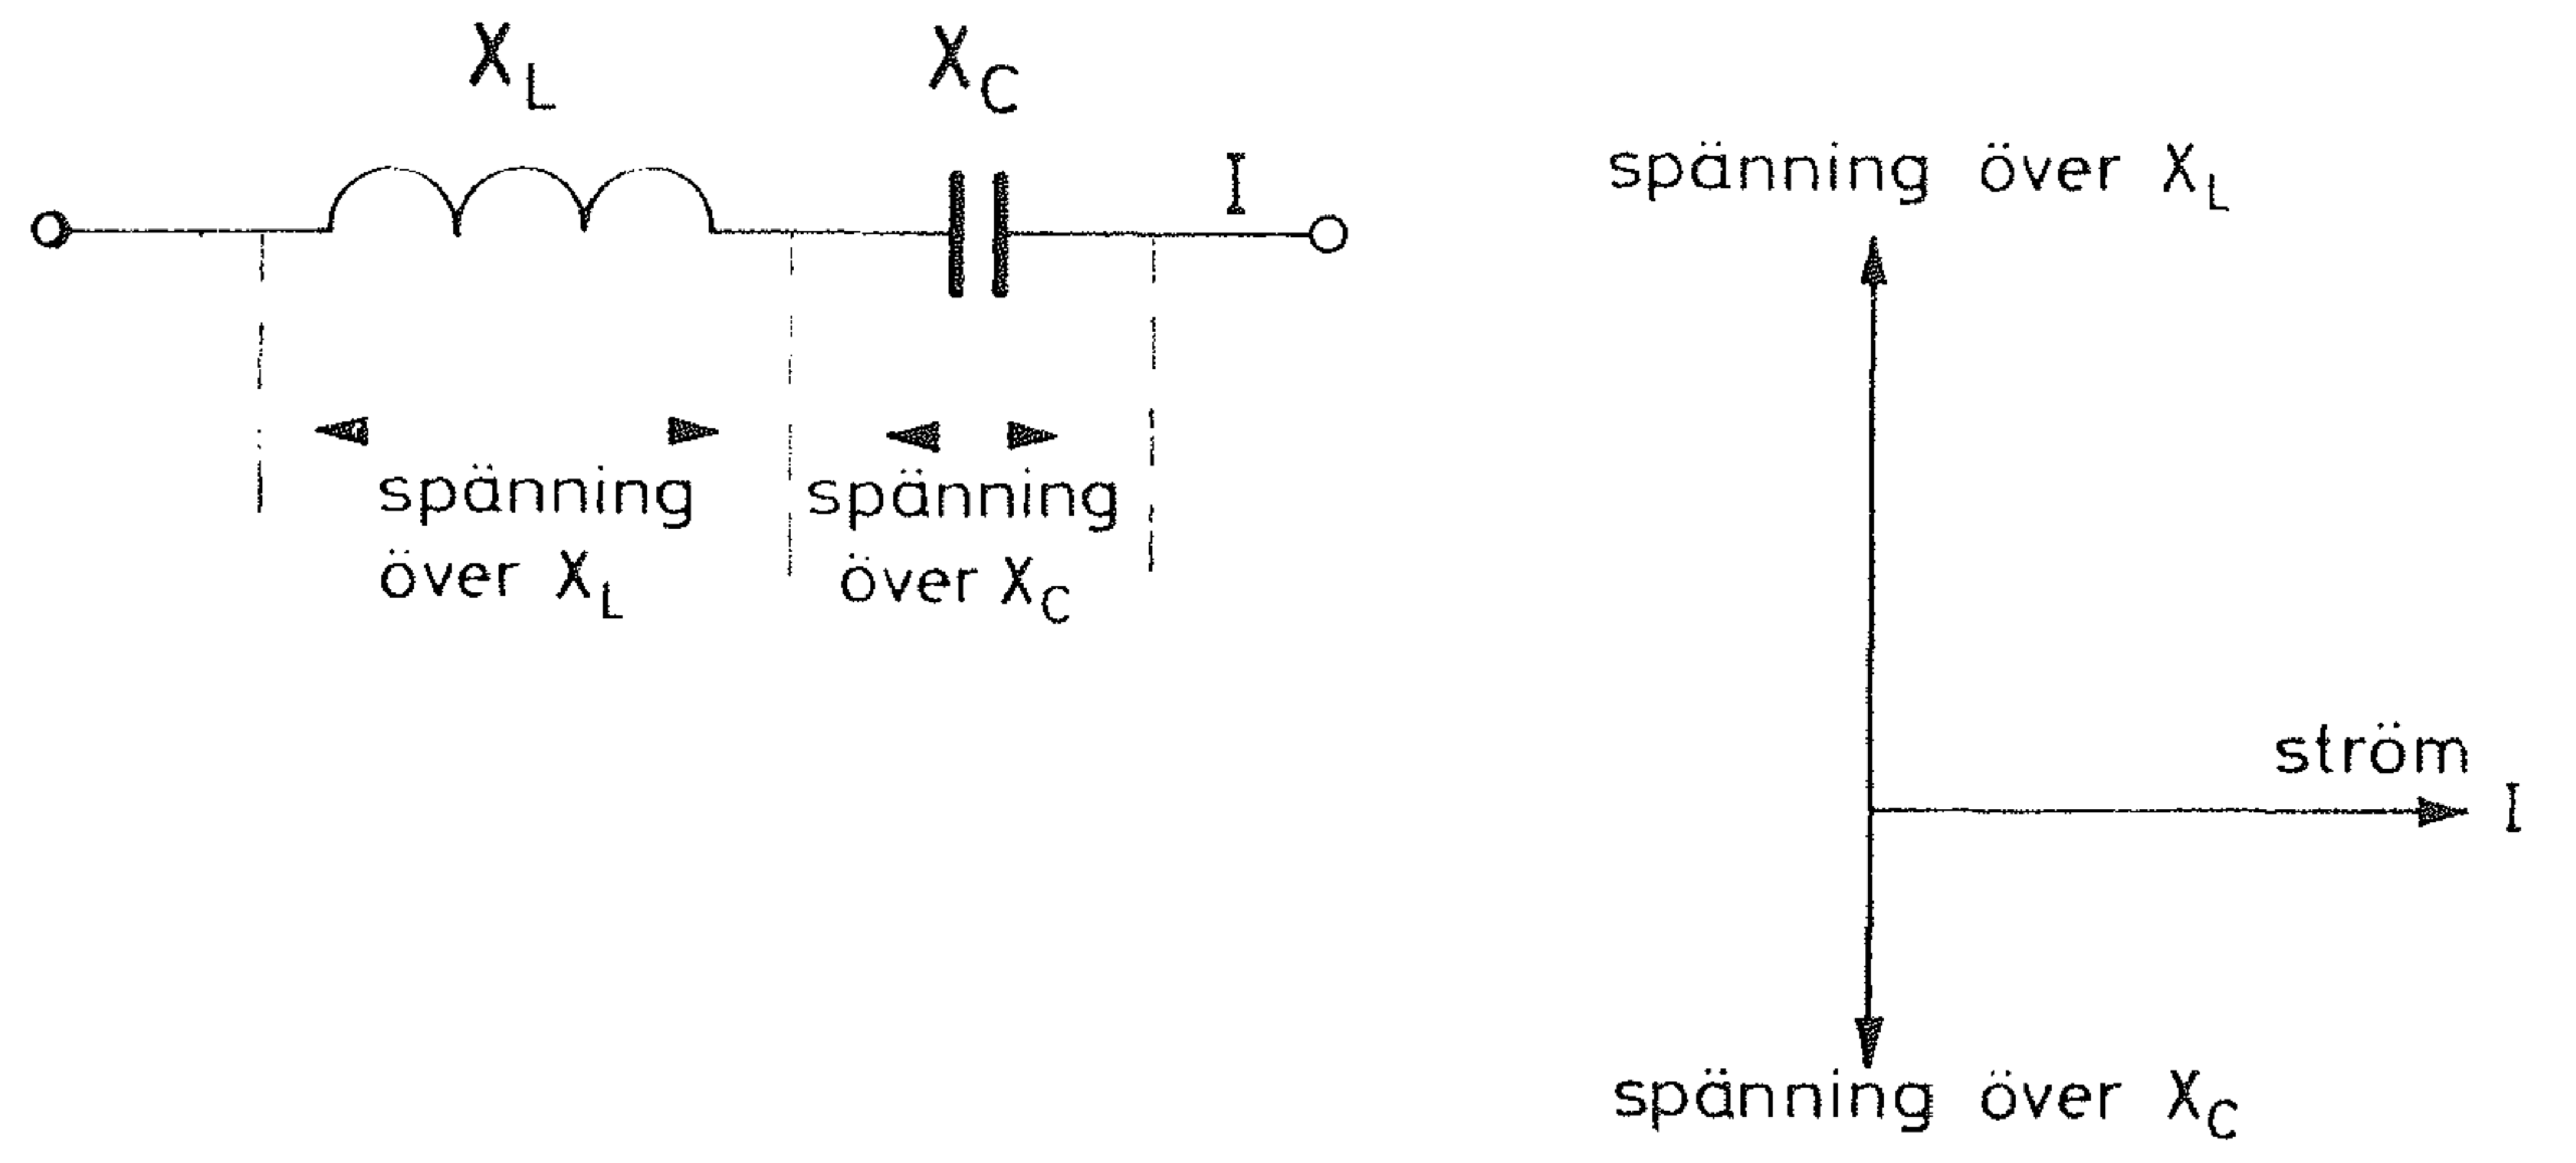
\includegraphics[width=\textwidth]{images/cropped_pdfs/bild_2_3-16.pdf}
\caption{Seriekopplad LC-krets}
\label{fig:BildII3-16}
\end{figure}

En seriekopplad LC-krets i bild \ref{fig:BildII3-16} ansluts till
växelspänningen \(U\) från en signalgenerator med inställbar frekvens \(f\).
Två fall studeras.

\textbf{Fall 1:} \(f = f_{res}\)

Signalgeneratorns frekvens \(f\) ställs lika med svängningskretsens
resonansfrekvens \(f_{res}\).
Impedansen \(Z\) i en seriekrets visar då ett mycket lågt värde mot generatorn.
Det flyter en stark ström i ledningen mellan generator och krets.

\textbf{Fall 2:} \(f < f_{res} \quad \text{eller} \quad f > f_{res}\)

Frekvensen \(f\) ställs lägre eller högre än kretsens resonansfrekvens
\(f_{res}\).

Eftersom svängningskretsen då visar hög impedans \(Z\) mot generatorn, så
flyter endast en svag ström i ledningen mellan generator och krets.

I praktiken finns även en resistans i serie med induktansen liksom en
parallellt över kapacitansen.
För enkelhetens skull bortses här från dessa resistanser.

Strömmen \(I\) är samma genom hela kretsen och strömvektorn \(I\) används
därför som så kallad riktfas.
Den ritas i bilden åt höger.
Om serieresistansen \(R\) varit med, så skulle ett spänningsfall \(U_R\) varit
inritad i samma riktning som \(I\) (i fas med \(I\)).
Spänningen över reaktansen \(X_C\) ligger 90\degree~efter \(I\) och ritad
rakt neråt (vektorerna roterar motsols).
Spänningen över reaktansen \(X_L\) (induktorn) ligger 90\degree~före \(I\) och
ritad rakt uppåt.

\subsection{Thomsons svängningskrets}
\textbf{HAREC a.\ref{HAREC.a.3.2.4}\label{myHAREC.a.3.2.4}}
\index{Thomson svängningskrets}
\index{svängningskrets}
\index{oscillator}
\index{oscillator!Thomson svängningskrets}

\begin{figure*}[ht]
\begin{center}
  %%\begin{wrapfigure}[30]{R}{0.5\textwidth}
  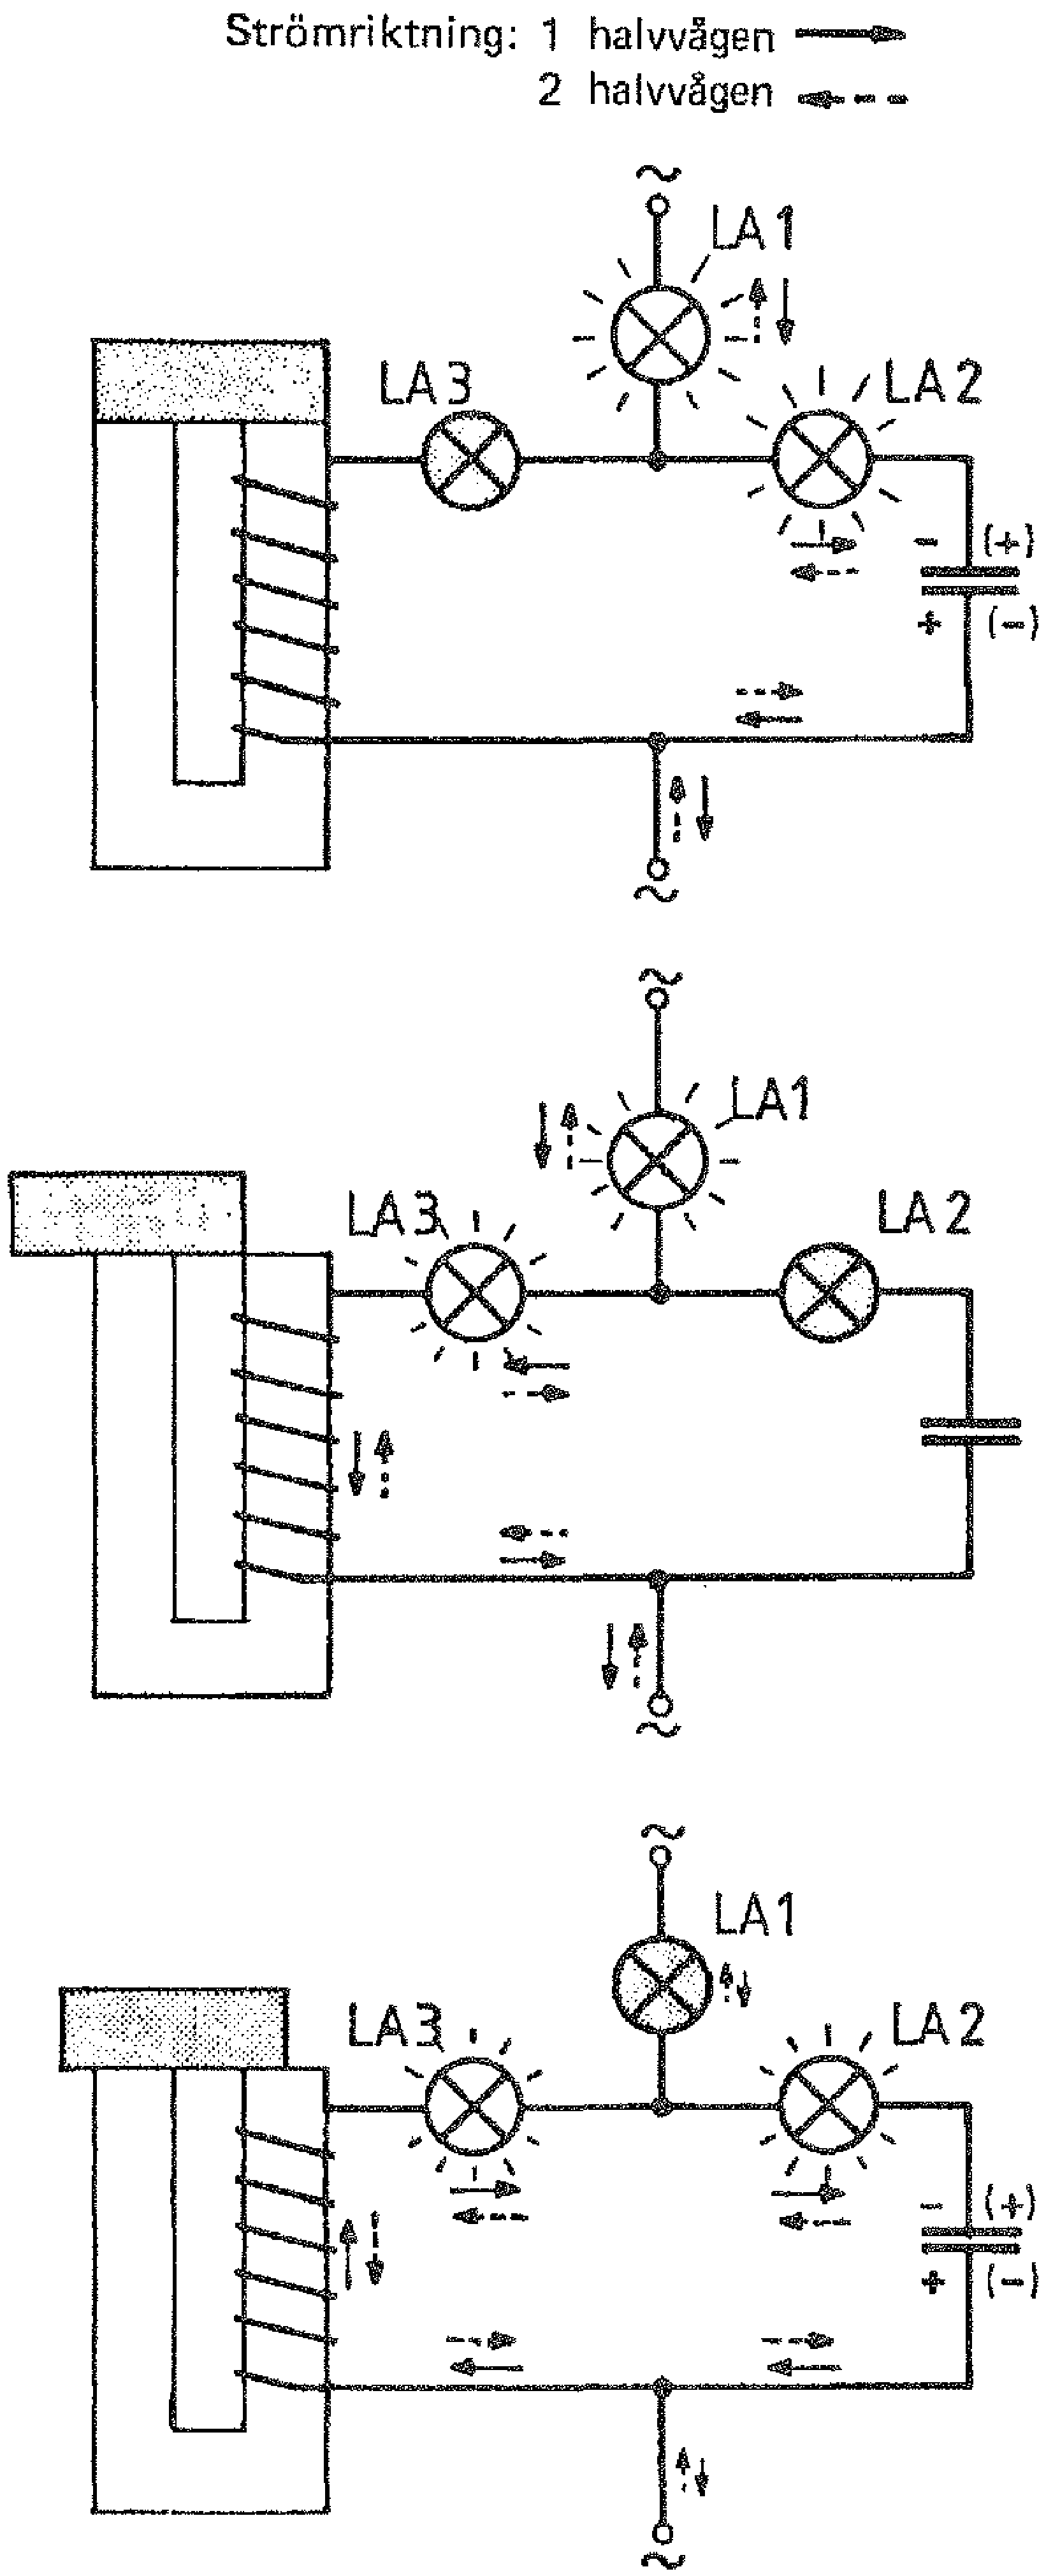
\includegraphics[width=0.4\textwidth]{images/cropped_pdfs/bild_2_3-17.pdf}
  \caption{Thomsons svängningskrets}
  \label{fig:BildII3-17}
  %%\end{wrapfigure}
\end{center}
\end{figure*}

Bild \ref{fig:BildII3-17} visar en svängningskrets, som består av en
kondensator och en induktor med förskjutbar järnkärna.
En ändring av kärnans tvärsnitt ändrar den magnetiska ledningsförmågan och
därmed induktansen.

Med anordningen kan resonansfrekvensen alltså ställas in så att den blir högre,
lika med eller lägre än den anslutna spänningens frekvens.
Tre fall undersöks:
\begin{enumerate}
\item \(X_L > X_c\) LA1 och LA2 lyser upp, en kraftig ström flyter genom
  kondensatorn,
\item \(X_L < X_C\) LA1 och LA3 lyser upp, en kraftig ström flyter genom
  induktorn,
\item \(X_L= X_C\) LA2 och LA3 lyser upp, LA1 lyser inte, en kraftig ström
  flyter i kretsen men inte i tilledningarna
\item \(X_L = X_C\) kallas Thomsons svängningsformel, vilken beskriver
  resonansfallet
\end{enumerate}

Då är de induktiva och kapacitiva reaktanserna i kretsen lika stora och tar ut
varandra.
Kvar är kretsens resistans, vilken vi tills vidare betraktar som försumbar.

Således \(X_L = X_C\), där

\begin{gather*}
  X_L = 2\pi fL \quad \text{och} \\
  X_C = \frac{1}{2\pi fC} \quad \text{sätts in.} \\
  2\pi fL = \frac{1}{2\pi fC} \quad 4\pi ^2f^2LC = 1 \\
  f^2 = \frac{1}{4\pi ^2LC} \quad f = \frac{1}{2\pi \sqrt{LC}} \\
  f\text{ [Hz] }L\text{ [H] }C\text{ [F] } \\
\end{gather*}

Formeln gäller både för parallell- och seriekretsar.

\textbf{Räkneexempel:}

\[L = 100\ nH \quad C = 10\ pF \quad f =\ ?\]
\begin{align*}
  f &= \frac{1}{2\pi \sqrt{100 \cdot 10^{-9} \cdot 10 \cdot 10^{-12}}} \\
  &= \frac{1}{2\pi 10^{-9}} \\
  &= \frac{10^9}{2\pi } \\
  &\approx 159\ MHz
\end{align*}

\subsection{Impedansen i en resonant krets}
\textbf{HAREC
  a.\ref{HAREC.a.3.2.1}\label{myHAREC.a.3.2.1b}
  a.\ref{HAREC.a.3.2.2}\label{myHAREC.a.3.2.2b}
  a.\ref{HAREC.a.3.2.3}\label{myHAREC.a.3.2.3}
  a.\ref{HAREC.a.3.2.4}\label{myHAREC.a.3.2.4b}
}
\index{resonans!impedans}
\index{impedans!resonanskrets}

En enkel framställning görs av hur impedans, reaktans och resistans förhåller
sig inbördes när en svängningskrets är i resonans.
Som exempel används följande kretsdata: Induktans 200~\(\mu H\),
kapacitans 200~pF, förlustresistans 10~\(\Omega\).

\subsubsection{Resonansfallet i en parallellkrets}
\label{parallellresonans}
\index{parallellresonans}
\index{resonans!parallellkrets}

\begin{figure*}[ht]
\begin{center}
  %%\begin{wrapfigure}[25]{R}{0.5\textwidth}
  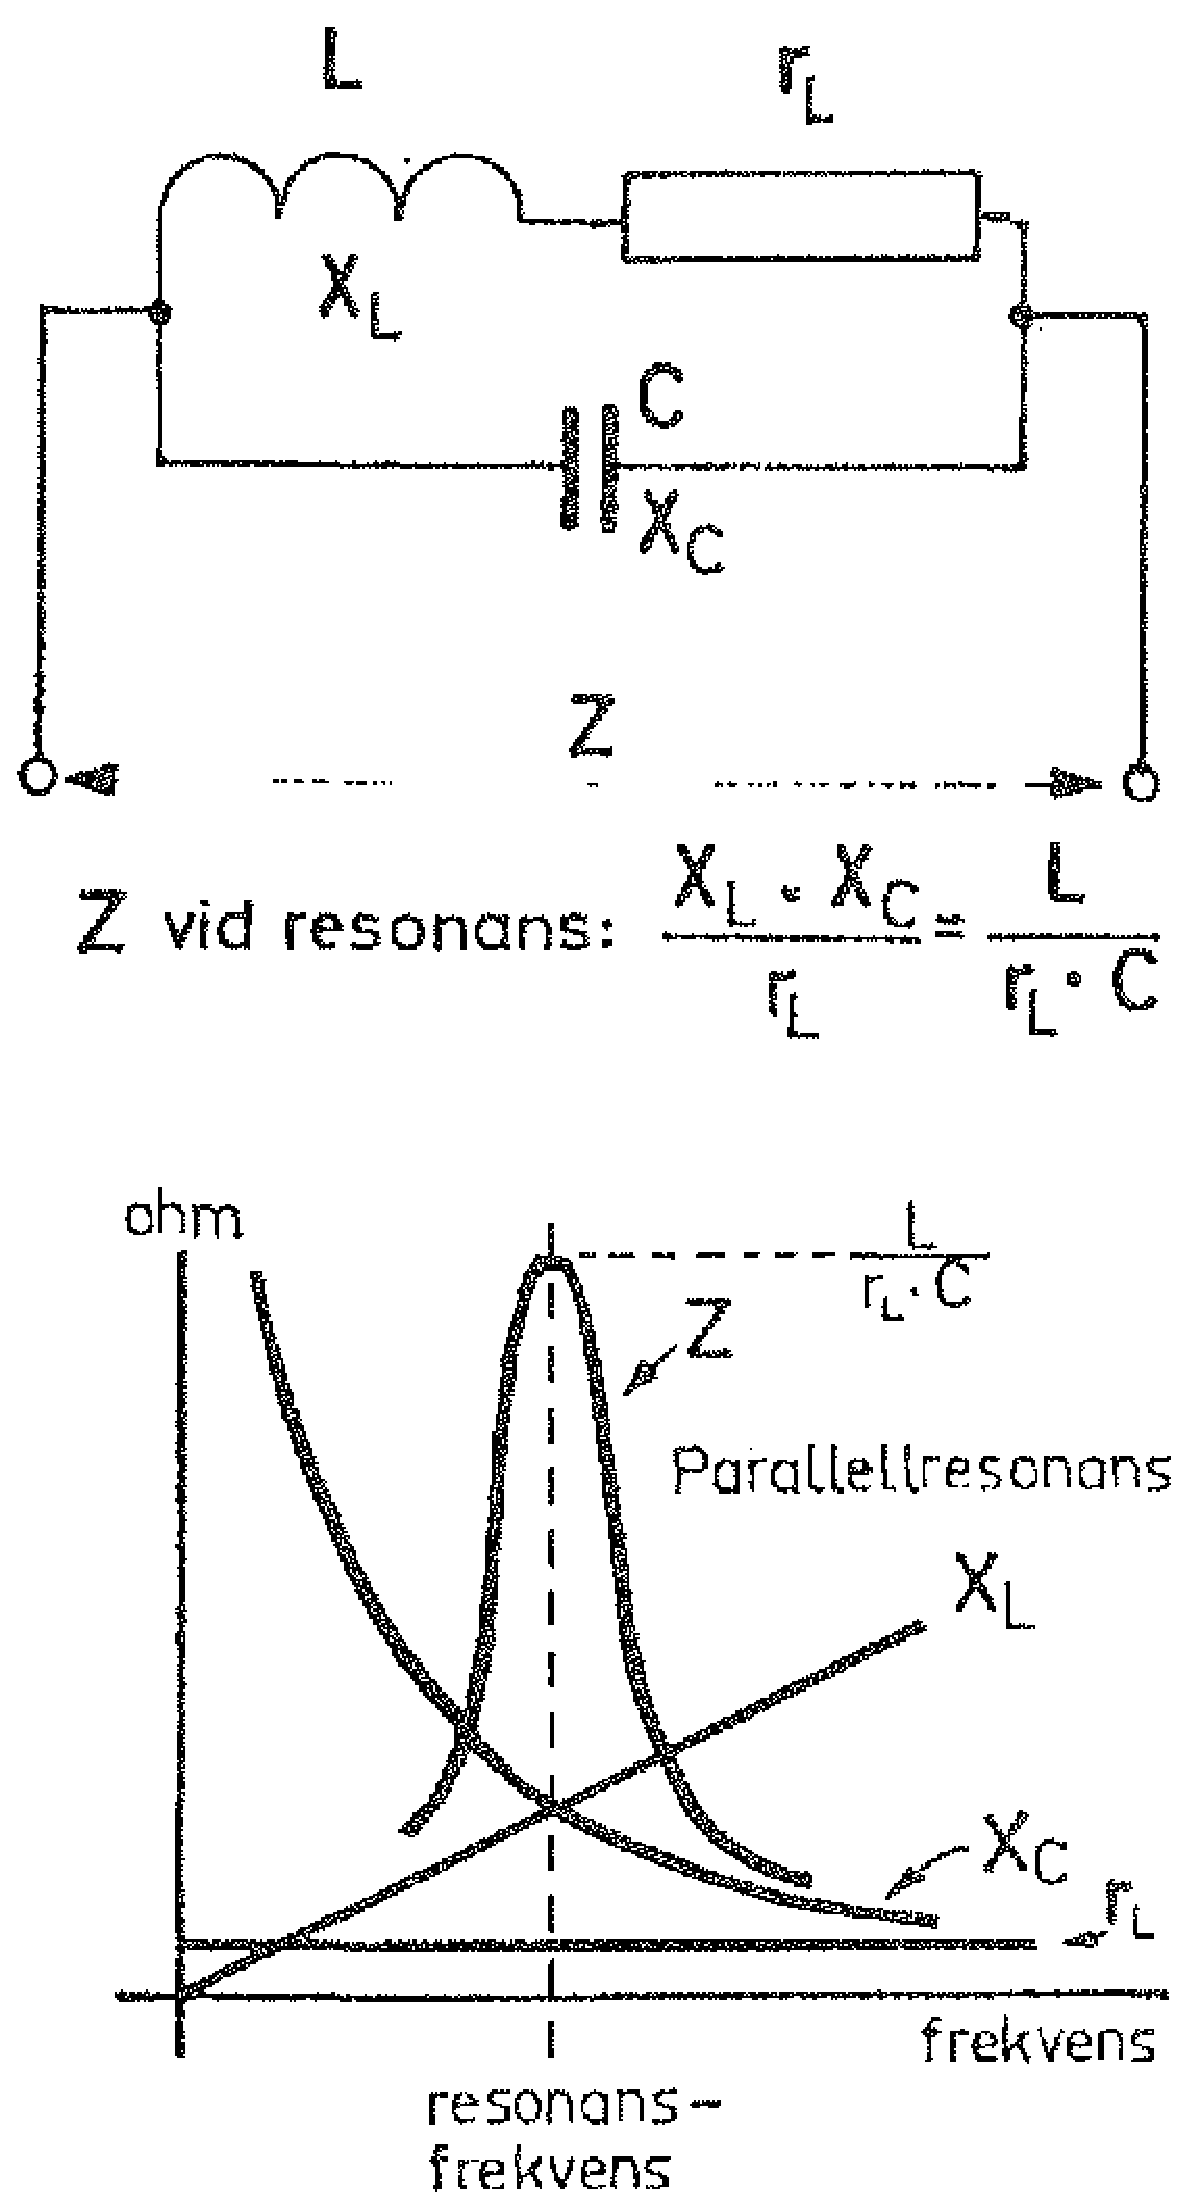
\includegraphics[width=0.5\textwidth]{images/cropped_pdfs/bild_2_3-18.pdf}
  \caption{Resonansfallet i parallellkrets}
  \label{fig:BildII3-18}
  %%\end{wrapfigure}
\end{center}
\end{figure*}

Parallellkretsen består i sig själv av seriekopplade komponenter, varav
\(X_L\) och \(X_C\) är reaktiva.
Vid resonans är dessa lika stora och motverkande.
Inom kretsen är således den resulterande reaktansen:

\[X_L - X_C = 0\]

Därför uppvisar samma krets en yttre reaktans av:

\[
  X = \frac{-X_L \cdot X_C}{X_L - X_C}
  = \frac{-X_L \cdot X_C}{0}
  = \infty
\]

I praktiken finns i kretsen också en resistans varför dessa extremvärden inte
uppstår.
Inne i en parallellkrets i resonans cirkulerar alltså en stark ström,
som endast begränsas av kretsens resistans.

Bild \ref{fig:BildII3-18} visar en parallellkrets där induktorn har resistansen
\(r_L\) och kondensatorn antas vara förlustfri.
Vidare förutsätts att kretsen är i resonans.

Vid resonans kan termen \(X_L - X_C = 0\) bytas mot \(r_L\) i formeln
\[X = \frac{-X_L \cdot X_C}{X_L - X_C}\] förutsatt att \(r_L\) är försumbart
jämfört med \(X_L\).

Därtill är \(X_L = 2\pi fL\) och \(X_C = \frac{1}{2\pi fC}\) det vill säga
\(X_L \cdot X_C = \frac{L}{C}\) som sätts in.

Parallellkretsens impedans vid resonans kan då skrivas

\[
Z = \frac{X_L \cdot X_C}{r_L} = \frac{L}{r_L \cdot C}
\]

Med ovanstående kretsdata blir Z = 100~k\(\Omega\).

Därav framgår, att impedansen i parallellkretsen är en funktion av det så
kallade L/C-förhållandet samt av kretsens resistiva förluster.

\subsubsection{Resonansfallet i en seriekrets}
\label{serieresonans}
\index{serieresonans}
\index{resonans!seriekrets}

\begin{figure*}[ht]
\begin{center}
  %%\begin{wrapfigure}[20]{R}{0.5\textwidth}
  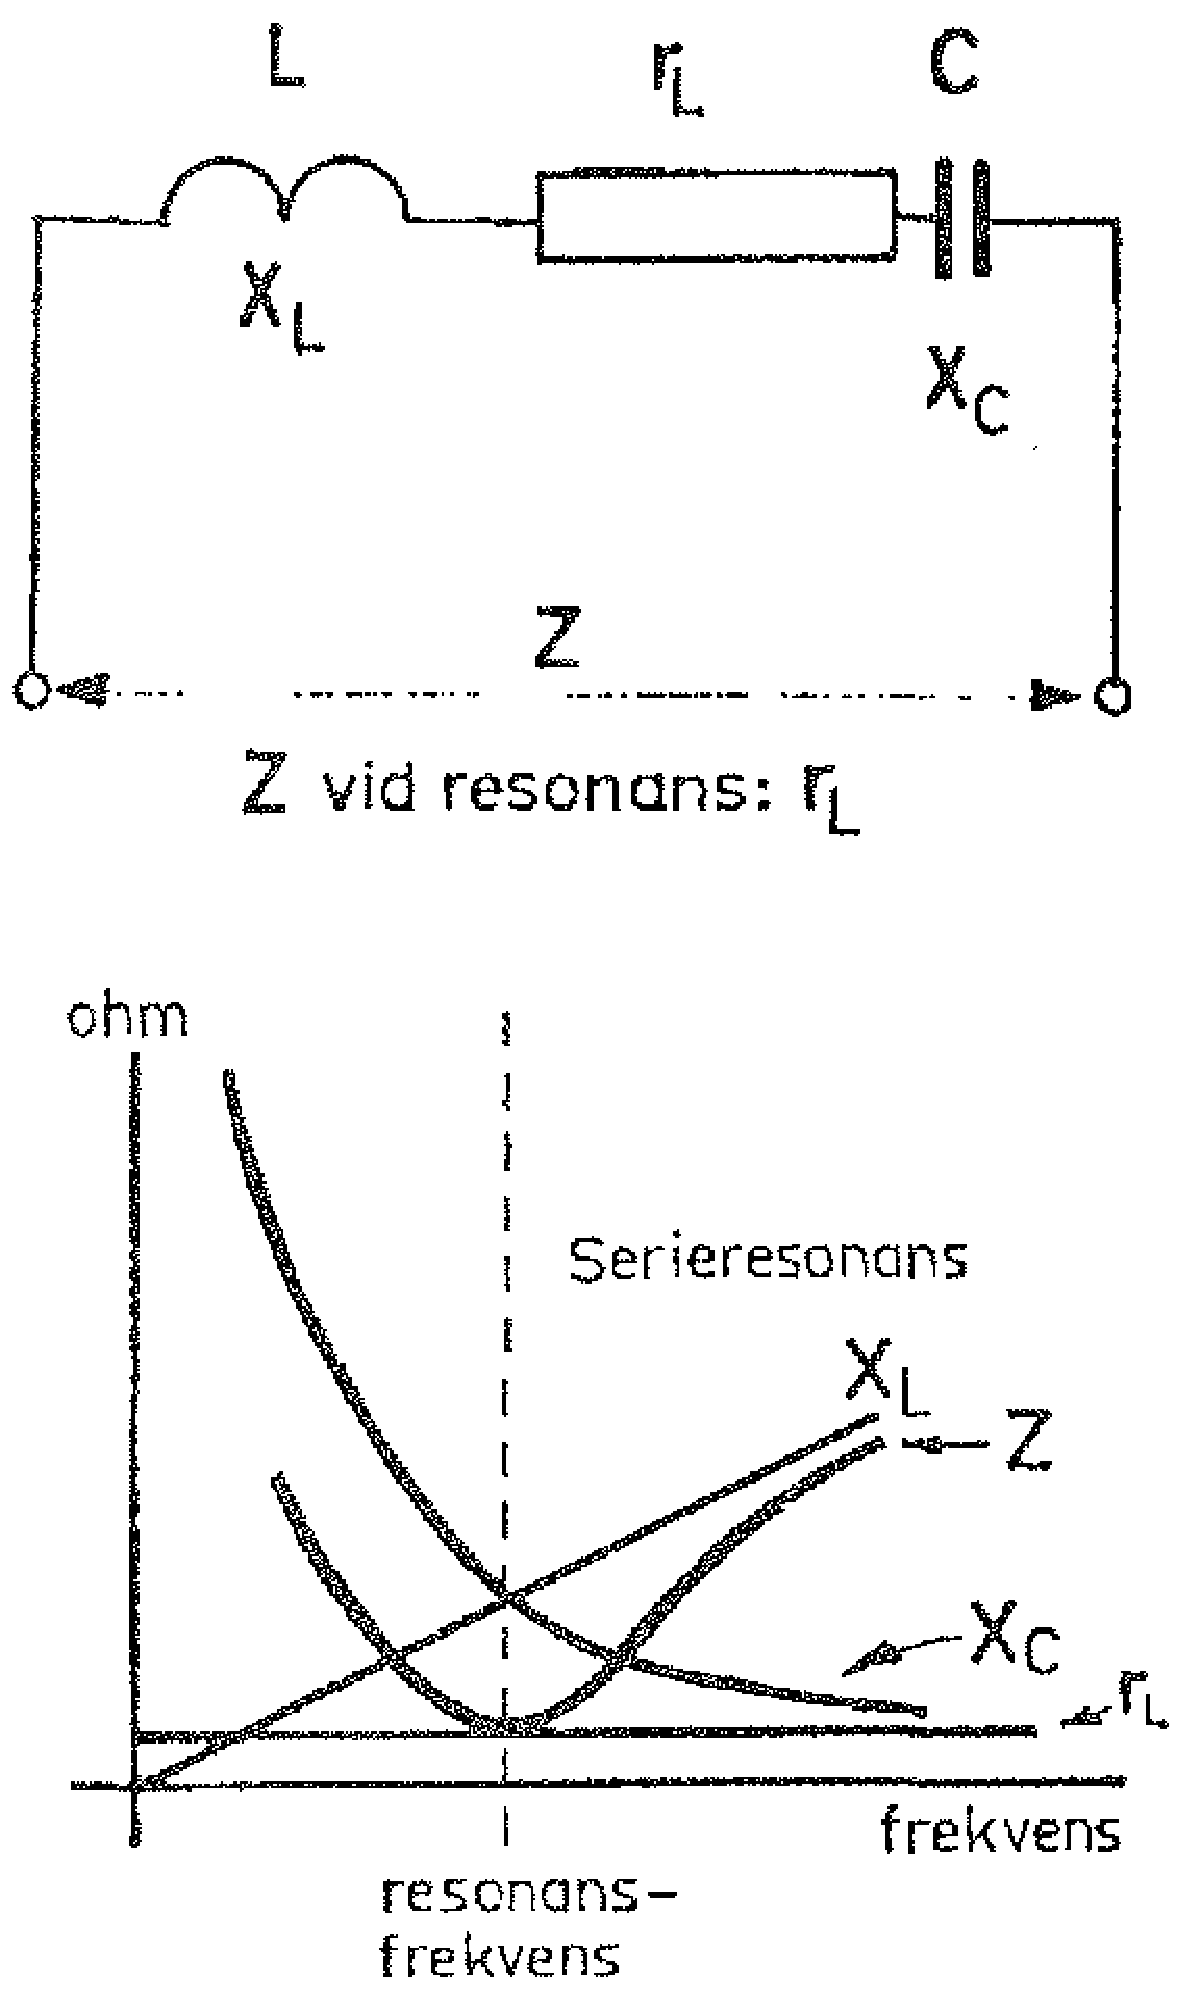
\includegraphics[width=0.5\textwidth]{images/cropped_pdfs/bild_2_3-19.pdf}
  \caption{Resonansfallet i seriekrets}
  \label{fig:BildII3-19}
  %%\end{wrapfigure}
\end{center}
\end{figure*}

Bild \ref{fig:BildII3-19} visar en seriekrets är i resonans, så är

\begin{align*}
& X_L = X_C \quad & \text{dvs.} \quad \omega L = \frac{1}{\omega C} \\
& \text{eller} & \\
& X_L - X_C = 0 \quad & \text{dvs.} \quad \omega L - \frac{1}{\omega C} = 0
\end{align*}

Med ovanstående kretsdata blir resonansfrekvensen:

\[
f_0 = \frac{1}{2\pi \sqrt{LC}} \approx 796\ kHz
\]

Vid resonansfrekvensen blir reaktansen 1000~\(\Omega\) både för induktansen och
kapacitansen.
Eftersom reaktansernas spänningsfall är motriktade tar de ut varandra.
Kretsens impedans i resonans blir resistansen \(r_L\) och
spänningsfallet över kretsen bestäms enbart av \(r_L\).

Antag att det alstras en spänning av 5~mV i antennkretsen.
Strömmen genom den vid resonans blir då \(\frac{5\ mV}{10\ \Omega} = 0,5\ mA\).

Av strömmen bildas reaktiva spänningar, det vill säga
\(0,5 mA \cdot 1000\ \Omega = 500\ mV\) både över induktans och kapacitans
(som tar ut varandra) och 5~mV över resistansen.

\subsection{Q-faktorn i en parallellkrets}
\textbf{HAREC a.\ref{HAREC.a.3.2.5}\label{myHAREC.a.3.2.5}}
\label{Q-faktor}
\index{Q-faktor}
\index{symbol!Q qualityfactor}

\begin{wrapfigure}[13]{R}{0.5\textwidth}
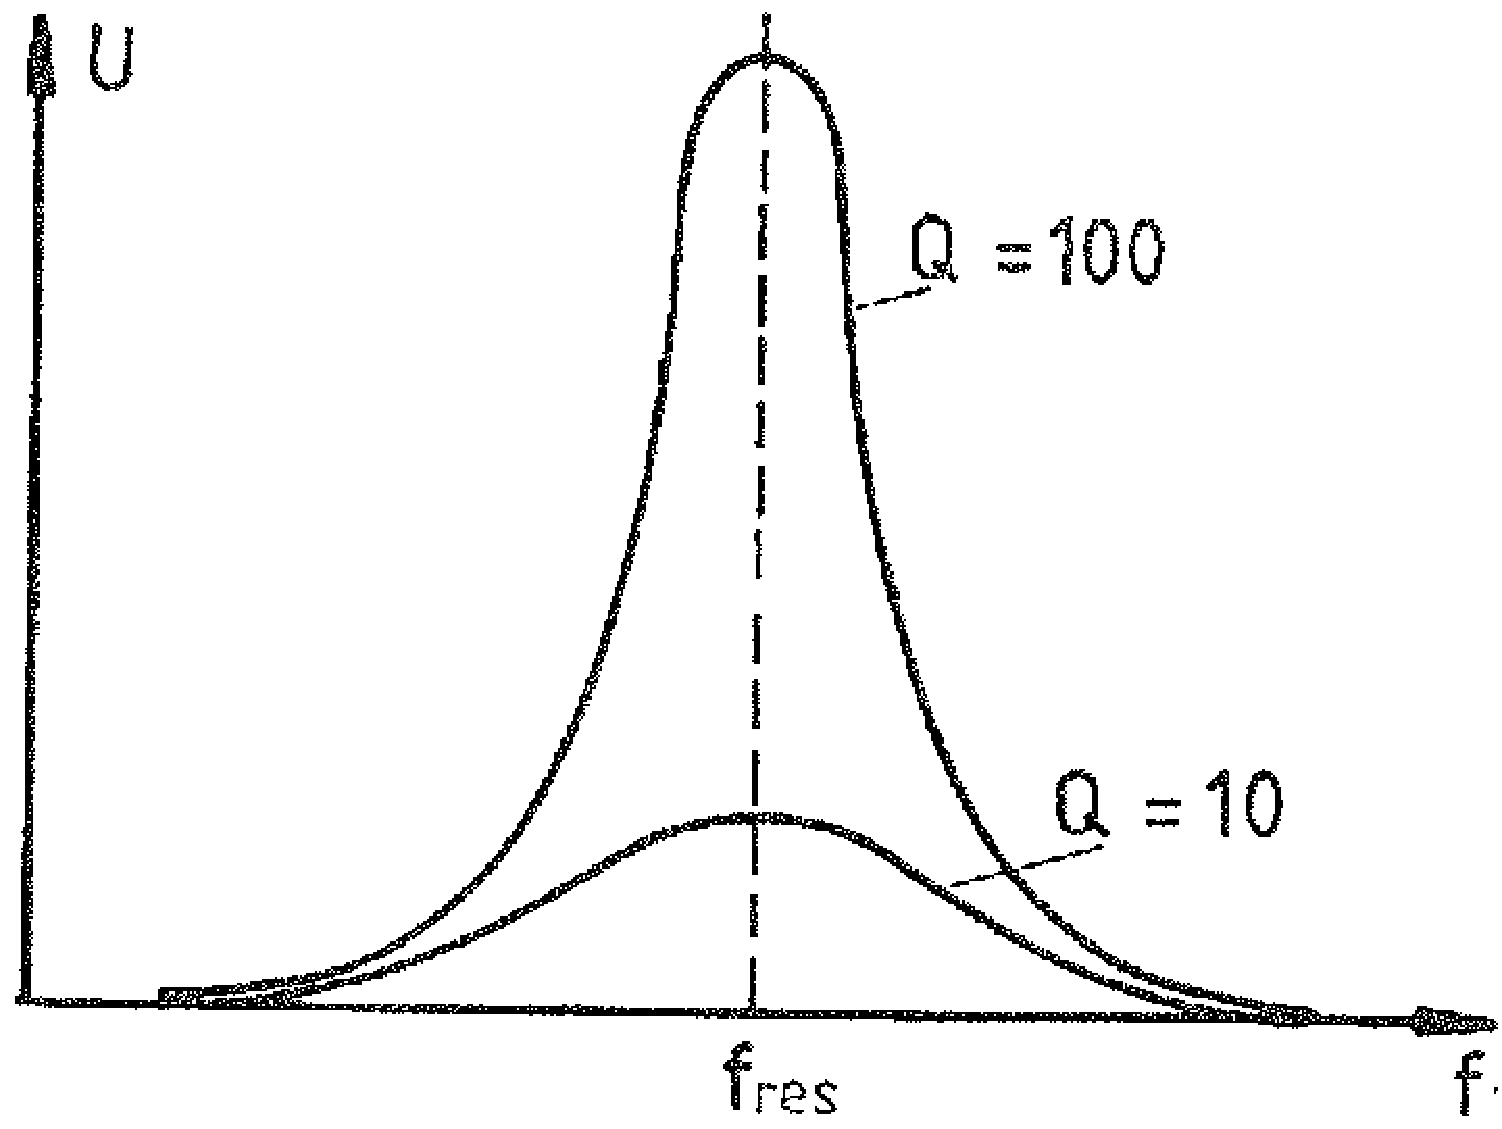
\includegraphics[width=0.5\textwidth]{images/cropped_pdfs/bild_2_3-20.pdf}
\caption{Q-värden i parallellkrets}
\label{fig:BildII3-20}
\end{wrapfigure}

Bild \ref{fig:BildII3-20} illustrerar Q-värden för parallellkrets.
Godhetstalet Q (=Quality Factor) kan ses som den förmåga en svängningskrets har
att lagra energi, det vill säga förhållandet mellan den lagrade energin och
energiförlusten i kretsen.
Energiförlusten yttrar sig som värmeutveckling.

\[
Q = 2\pi \frac{\text{lagrad energi i kretsen}}{\text{energiförlusten per period}}
\]

Energiförluster uppstår både i kretsens kondensator och induktor, men moderna
kondensatorer har så låga förluster att induktorn ensam kan anses bestämma
Q-värdet, åtminstone i kortvågsområdet.

En växelspänning \(U_1\) ansluts till en parallellkrets.
I resonansfallet uppträder då en spänning \(U_2\) över kondensatorn och
induktorn.

\(U_2\) är mycket större än \(U_1\).
Ju högre \(Q\) är i kretsen desto större är förhållandet mellan \(U_2\) och
\(U_1\).

I kortvågsområdet är det vanligt med ett \(Q\) i storleksordningen 30--100.
Ju högre Q är, desto mindre är bandbredden.

När svängningskretsen är i resonans gäller sambandet

\[Q = \frac{f_{res}}{b}\]

Bandbredden ökar (avstämningsskärpan minskar) vid ökande frekvens på grund av de
större kretsförlusterna.

\begin{wrapfigure}{R}{0.5\textwidth}
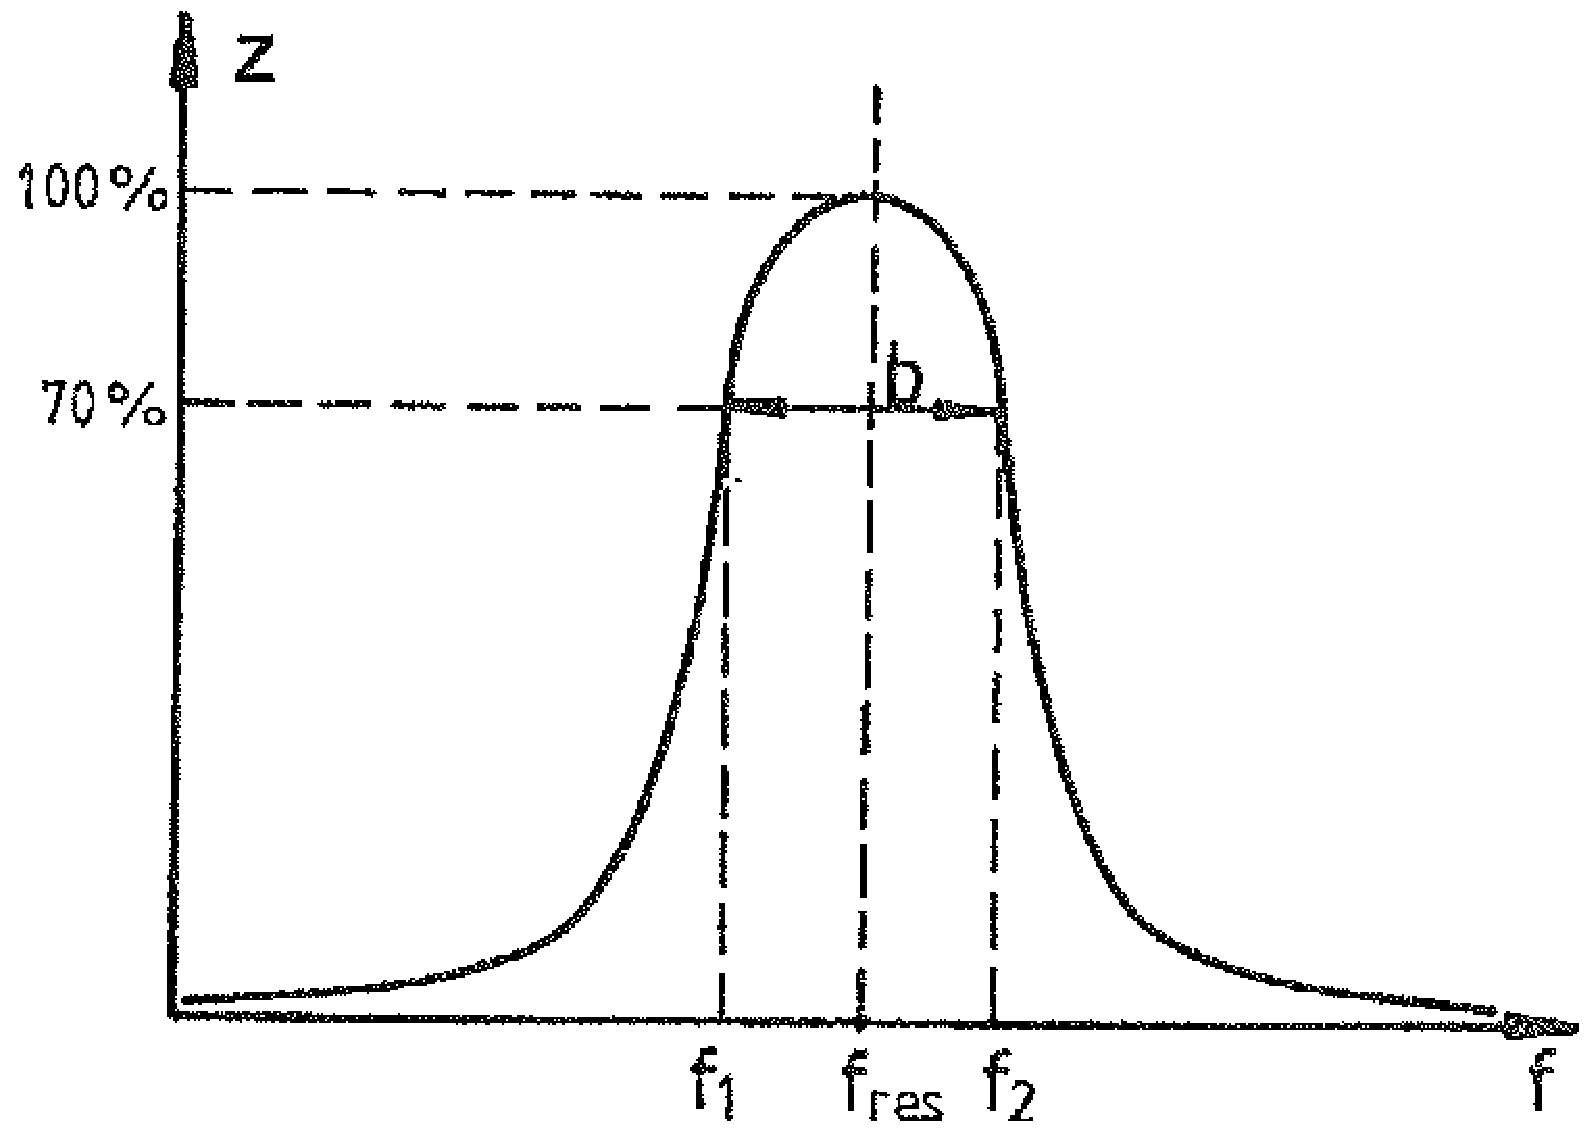
\includegraphics[width=0.5\textwidth]{images/cropped_pdfs/bild_2_3-21.pdf}
\caption{Bandbredd i parallellkrets}
\label{fig:BildII3-21}
\end{wrapfigure}

\subsection{Bandbredd}
\textbf{HAREC a.\ref{HAREC.a.3.2.6}\label{myHAREC.a.3.2.6}}
\index{bandbredd}

Bild \ref{fig:BildII3-21} visar med en kurva vilket impedansvärde kretsen har
vid olika frekvenser.
Impedansens högsta värde är vid frekvensen \(f_{res}\) och avtar vid frekvenser
som är högre eller lägre.
Vid frekvenserna \(f_1\) och \(f_2\) är impedansvärdet till exempel 70~\% av
maximalvärdet.
Med bandbredden \(b\) förstås skillnaden mellan impedansvärdena i ett sådant
frekvenspar, det vill säga \(b = f_2 - f_1\).
